%======================================================================
\chapter{Cutting Through the Noise: Using Deep Neural Network Metamodels for High Dimensional Nested Simulation}
\label{chap:project2}
%======================================================================


\section{Introduction}

Deep neural networks~\citep{hastie2009elements,lecun2015deep} have attracted attentions of researchers and practitioners due to their success in solving real-world machine learning tasks such as AlphaGo~\citep{silver2016mastering} and ChatGPT~\citep{chatgpt}.
Since the first artificial neural network model~\citep{mcculloch1943logical} and the first algorithm for training a perceptron~\citep{rosenblatt1958perceptron}, especially after the introduction of backpropagation~\citep{rumelhart1985learning} and the growth of high-performance computing, the field of artificial neural network and deep learning in general has grown rapidly.
Two specialized neural network architectures that are relevant to our study are recurrent neural networks (RNNs)~\citep{williams1989learning,sutskever2014sequence} and long-short-term memory (LSTM)~\citep{hochreiter1997long,chung2014empirical}, as we need to train metamodels\footnote{In the field of actuarial science, a metamodel is commonly referred to as a proxy model.} that take sequential observations as input.
Despite their success, deep neural network models are often criticized for their lack of transparency and interpretability, which hinders their adoption in financial and actuarial applications.
Enormous research efforts are spent to test and improve the robustness of deep neural network models with carefully designed noise injection methods.
~\cite{poole2014analyzing} show that injecting synthetic noise before and after hidden unit activations during training improves the performance of autoencoders.
~\cite{neelakantan2015adding} improve learning for deep neural networks by injecting synthetic noise to the gradients during backpropagations.
A branch of research has been devoted to understanding the resilience of neural network models to noise in training labels.
For example,~\cite{luo2016understanding} show that adding synthetic label noise to the convolutional neural network (CNN) can improve its ability to capture global features. 
~\cite{srivastava2014dropout} quantify the error tolerance by injecting synthetic label noise with a custom Boltzmann machine hardware.
~\cite{szegedy2013intriguing} find that neural networks are vulnerable to adversarial examples, and~\cite{goodfellow2014explaining} design an efficient method to generate such noisy examples to exploit the vulnerability to adversarial perturbations.
~\cite{carlini2017towards} design targeted attacks to training labels to test the robustness of neural networks. 
Instead of using synthetic noise, ~\cite{jiang2020beyond} inject real-world label noise and examine noise tolerance of neural networks with controlled noise levels.
The aforementioned studies use real-world data, as is typically the case for many neural network studies, where noise is already present in the training labels before any noise injection.
Users of real-world data have little control over the noise level of the original training labels and usually examine the effect of noisy data by injecting noise, but it is unclear whether a neural network model trained on noisy data actually learns the real, i.e., noiseless, feature-label relationship.
Due to their lack of transparency and interpretability, the adoption of deep neural networks in financial and actuarial applications has been received by regulators with some skepticism.

The contributions of our study are two-fold:
\begin{enumerate}
    \item We study what deep neural networks learn from noisy data by training them using simulated data based on well-designed simulation experiments.
    This is a novel way to study the effect of noisy data and error tolerance of neural network models as one can \textit{reduce noise} in the data by increasing the number of replications in a simulation model.
    This new way of studying neural network models can provide more direct evidence on their transparency and interpretability.  
    \item We propose two generic nested simulation procedures that uses deep neural networks as metamodels to improve its efficiency while maintaining transparency. 
    In essence, a pilot stage simulation is used to generate a large number of noisy data, which are then used to train a metamodel.
    Depending on the application, a trained metamodel can serve two purposes: (1) to identify a set of tail scenarios, and (2) to estimate risk measures directly.
    The first procedure uses a metamodel to identify a set of potential tail scenarios on which computations are performed in the second stage, while the second procedure uses metamodel predictions to estimate risk measures directly.
    Our numerical results show that deep neural network metamodels can identify the tail scenarios accurately and so the proposed procedures can estimate tail risk measures with similar accuracy while, at the same time, using less simulation budget.
\end{enumerate}


We are curious about fundamental questions like ``What do deep neural networks learn from noisy data?'' and ``How well do neural networks learn from noisy data?''.
Data-driven answers to these questions prevail in the existing literature.
In supervised learning, deep neural networks are believed to learn from the given data about the feature-label relationship to predict new labels for unseen features.
Cross validation using to assess a subset, i.e., the validation set, of the original data, is a common way to access the quality of learning.
Generalization error on the test labels is another popular assessment metric.
But the test set is also a subset of the original data.
In this study, we revisit these questions in a simulation context and propose an alternative approach to answer them.
Instead of relying solely on real-data (splitting it into multiple subsets), we propose using stochastic simulation outputs as training labels for deep neural network models.
By controlling the simulation design parameters, such as the number of independent replications, we can control the quality (and also the quantity) of the training labels fed into the neural networks.
In such a controlled environment, we obtain more clear-cut answers to the above fundamental questions.

In nested simulation, a simulation model is used to generate a large number of outer scenarios, and each scenario is then used as an input to another simulation model.
Borrowing terminologies from machine learning research, we can view a set of simulated outer scenarios and the estimated hedging errors for those scenarios as the \textit{features} and (noisy) \textit{labels}.
One can train supervised learning models using these simulated features and labels.
They are then used to replace the time-consuming inner simulations by the trained model.
We refer to the trained supervised learning models as \textit{metamodels} of the inner simulation, which is also known as the \textit{surrogate models}.
Metamodeling is a popular approach to reduce the computational burden of simulation-based applications by replacing the time-consuming simulation with a metamodel.
The metamodel is trained using a set of simulated data, and it is used to predict the simulation output for new inputs.
The study of metamodeling is an active research area in the simulation literature, and using deep neural networks as metamodels is a relatively new development.
~\cite{fonseca2003simulation} provide general guidelines for simulation metamodeling with neural networks,~\cite{lieu2022adaptive} use deep neural networks as metamodels of a simulation model for structural reliability analysis, and~\cite{salle2014efficient} show that neural network metamodels help achieve higher prediction accuracy that other metamodels in approximating agent-based simulation models.
A popular metamodel in nested simulation procedures is stochastic kriging.
~\cite{liu2010stochastic} use stochastic kriging as a metamodel of Monte Carlo simulations to estimate the Conditional Value-at-Risk (CVaR) of a portfolio of derivative securities, and~\cite{gan2015valuation} use stochastic kriging for an efficient valuation of large portfolios of variable annuity (VA) contracts.
Other studies, such as ~\cite{broadie2015risk},~\cite{hong2017kernel}, and~\cite{zhang2022sample} use regression, kernel smoothing, and the likelihood ratio method, respectively.
Our study has three key distinctions over the existing ones:
\begin{enumerate}
    \item  our metamodel has high-dimensional inputs. In machine learning terminology, the features are high-dimensional vectors.
    To estimate the hedging error of a typical VA contract, the number of features is in the order of hundreds, which is at least one order of magnitude larger than the number of features in the aforementioned studies,
    \item  for estimating tail risk measures, our metamodel is only used for tail scenario identification but is \textit{not} used in the estimation of the tail risk measures.
    This is a feature designed particularly to convince regulators that the losses used in estimating the risk measure are based on a transparent inner simulation model rather than on some black-box metamodels, and
    \item  using simulation models as data generators, we can decrease the noise level and get arbitrarily close to the true labels by increasing the number of replications in the simulation model.
    This design allows a systematic study of the effect of noisy training labels on the performance of neural network models in predicting the noiseless labels.
\end{enumerate}

The rest of this article is organized as follows: 
% Section~\ref{sec2:problem-formulation} presents the problem settings for tail risk measures and dynamic hedging of VAs. 
% Section~\ref{sec2:metamodel2Stage} proposes an efficient two-stage nested simulation procedure that uses deep neural networks as metamodels to help reduce simulation budget by only performing computations on identified tail scenarios. 
% Section~\ref{sec2:metamodel1Stage} proposes a one-stage nested simulation procedure that estimates risk measures directly with metamodel predictions.
% Section~\ref{sec2:numerical} demonstrates the efficiency of deep learning proxies and examines error tolerance of two LSTM metamodels with different numbers of trainable parameters. 
% Practical suggestions are provided for the choice of suitable metamodels and simulation settings. 


\section{Problem Formulation} \label{sec2:problem-formulation}

In this section we present notations, problem settings, and a simulation model for risk estimation for hedging errors of variable annuities.
A main goal of the section is to showcase the complexity of the simulation model, which we use as a data generator to train deep neural network metamodels (Section~\ref{sec2:metamodel2Stage} and Section~\ref{sec2:metamodel1Stage}).
For readers who are interested in the examination of a neural network metamodel, it is sufficient to understand that our simulation model generates data with 240 features and 1 real-value label and our metamodels are generally applicable to any simulation model that generates data with similar characteristics.

\subsection{Tail Risk Measures: VaR and CVaR}
Measuring and monitoring risks, particularly tail risks, are important risk management tasks for financial institutions like banks and insurance companies.
Two most popular tail risk measures are VaR and CVaR~\citep{hardy2022quantitative, rockafellar2002conditional}. 

Consider a loss random variable $L$ whose losses and gains lie in the right and left tails, respectively, of its distribution.
For a given confidence level $\alpha\in [0,1]$, the $\alpha$-VaR and $\alpha$-CVaR are defined in Equation~\eqref{eq1:var} and Equation~\eqref{eq1:cvar}, respectively.
Tail risk measures like VaR and CVaR are widely used for setting regulatory and economic capital, which is the amount of capital a financial institution holds to cover its risk.
For example, European insurers set regulatory capital at $99.5\%$-VaR according to Solvency II~\cite{eiopa2014underlying}.
In Canada, the regulatory capital requirement for VAs is set based on CVaRs as prescribed in~\cite{osfi2017life}.

Let $L_1,L_2,\ldots,L_M$ be $M$ independent and identically distributed (i.i.d.) simulated losses of $L$ and let $L_{(1)}\leq L_{(2)}\leq \ldots\leq L_{(M)}$ be the corresponding ordered losses.
For a given confidence level $\alpha$ (assume that $\alpha M$ is an integer for simplicity), $\alpha$-VaR can be estimated by the sample quantile $\widehat{\VaR}_\alpha = L_{(\alpha M)}$. Also, $\alpha$-CVaR can be estimated by
\begin{equation} \label{eq2:cvar-hat}
    \widehat{\CVaR}_\alpha = \frac{1}{(1-\alpha)M} \sum_{i=\alpha M + 1}^{M}L_{(i)} = \frac{1}{(1-\alpha)M} \sum_{i \in \tail_{(1-\alpha )M}}L_{i}.
\end{equation}
Equation \eqref{eq2:cvar-hat} is the same as \eqref{eq1:cvar-hat} except we define a \textit{true tail scenario set} of size $k$ as $\tail_{k} = \{i: L_i > L_{(M-k)}\}$.
In this study, the loss random variable of interest is the hedging error for VA.

\subsection{Simulation Model for Variable Annuity Payouts}\label{subsec:VApayout}

Variable annuity contracts offer different types of guarantees.
Generally speaking, a portion of the VA premium is invested in a sub-account whose return is linked to some stock indices.

Two relevant types of guarantees in our studies are:
\begin{itemize}[noitemsep]
    \item \textbf{Guaranteed Minimum Maturity Benefit (GMMB)}: A GMMB contract pays a maturity benefit equal to the greater of the sub-account value and a fixed guarantee value.
    The guarantee value is often set as a percentage, e.g., 75\% or 100\%, of the initial premium.

    \item \textbf{Guaranteed Minimum Withdrawal Benefit (GMWB)}: A GMWB contract guarantees the minimum amount of periodic withdrawal the policyholder can take from the sub-account until maturity, even if the sub-account value reduces to zero.
    The minimum withdrawal benefit is typically a fixed percentage of the guarantee value.
    The guarantee value will decrease if the withdrawal exceeds the guaranteed minimum. The GMWB is typically offered with an accumulation period, during which no withdrawals are made but a GMDB is usually offered. Additional features offered with the GMWB include roll-up, ratchet, and reset~\citep{geneva2013variable}.
\end{itemize}
For a comprehensive review of other types of VA contracts such as Guaranteed Minimum Death Benefit (GMDB), Guaranteed Minimum Accumulation Benefit (GMAB) and Guaranteed Lifetime Withdrawal Benefit (GLWB), we refer readers to~\cite{hardy2003investment}.
Next we present a summary of dynamic hedging for VA contracts.
We refer readers to~\cite{dang2021efficient} for detailed modeling of insurer liabilities in different VA contracts and Greek estimation.

Consider a generic VA contract with maturity $T>0$ periods, e.g., $T=240$ months.
Denote the policyholder's (random) time of death by $\tau>0$.
Then the contract expires at $T'=\min\{T,\tau\}$, i.e., the earlier of the contract maturity and the death of the policyholder.
Let $S_t$, $F_t$, and $G_t$ be the indexed stock price, the subaccount value and the guarantee value, respectively, at time $t=1,2,\ldots,T$.
Evolution of the subaccount value and the guarantee value of a VA contract affect the contract payout.
Note that the policyholder's (random) time of death also affects the timing of the benefit payout for certain types of VA such as GMDB, but this is not considered in our study for simplicity.
For clarity, we use $F_t$ and $F_{t_+}$ to denote the sub-account value just before and just after the withdrawal at time $t$, if any.
Let $\eta_g$ be the gross rate of management fee that is deducted from the fund value at each period and let $\eta_n < \eta_g$ be the net rate of management fee income to the insurer.
The difference between the gross management fee and the net management fee income represents the incurred investment expenses.

At the inception of the contract, i.e., $t=0$, we assume that the whole premium is invested in the stock index and the guarantee base is set to the sub-account value:
\begin{equation*}
    S_0=F_0=G_0.
\end{equation*}
At each time $t=1,\ldots,T$, the following events take place in the following order:
\begin{enumerate}
    \item The sub-account value changes according to the growth of the underlying stock and the (gross) management fee is deducted. That is, 
        \begin{equation*}
            F_t = F_{(t-1)_+}\cdot\frac{S_{t}}{S_{t-1}}\cdot(1-\eta_g),
        \end{equation*} 
    where $(x)^+=\max\{x,0\}$ and $F_{(t-1)_+}$ will be defined later. The insurer's income at time $t$ is the net management fee, i.e., $F_t\eta_n$. 

    \item The guarantee value ratchets up (ratcheting is a common feature in GMWB) if the sub-account value exceeds the previous guarantee value, i.e., 
        \begin{equation*}
            G_t = \max\{G_{t-1},F_t\}.
        \end{equation*} 

    \item The withdrawal is made (for GMWB) and is deducted from the sub-account value, i.e., 
        \begin{equation*}
            F_{t_+} = (F_t - I_t)^+,
        \end{equation*} 
    where $I_t = \gamma G_t$. A GMMB can be modeled with $\gamma = 0$.
\end{enumerate}

We see from the above modeling steps that the status of a generic VA contract is summarized by a triplet $(S_t,F_t,G_t)$ whose evolution is driven by the stochasticity of $S_t$.
In practice, the simulation model may also incorporate additional complications like mortality, lapse, and excess withdrawal, etc.

At any time $t=1,\ldots,T$, the insurer's liability in a VA contract is the present value of all payments, net of the fee income.
For example, suppose that the per-period risk-free rate is $r$, then
the insurer's time-$t$ liability for a GMMB contract is $V_t = e^{-r(T-t)}\cdot (G_T - F_T)^+ - \sum_{s=t+1}^{T} e^{-r(T-s)} F_s \eta_n$.
Also, the insurer's time-$t$ liability for a GMWB contract is $V_t = \sum_{s=t+1}^{T} e^{-r(T-s)} [(I_s - F_s)^+- \eta_n F_s] $.

For example, consider the time-$t$ liability $V_t$ of a GMWB:
Suppose that given the stock sample path, e.g., an outer path $S_1,\ldots,S_t$, one can simulate future stock prices $\Stilde_{t+1},\ldots,\Stilde_{T}$, e.g., inner sample paths, based on some asset model such as a Black-Scholes model.
The tilde symbol ($\sim$) over a quantity denotes its association with the inner simulation.
Given the time~$t$ state $(S_t,F_t,G_t)$, following~\cite{cathcart2015calculating} the sensitivity of $V_t$ with respect to $S_t$ can be estimated by a pathwise estimator~\citep{glasserman2004monte}:
\begin{align}\label{eq2:delta}
    \Delta_t(\Stilde_{t+1},\ldots,\Stilde_{T} | S_t) = \frac{\partial V_t}{\partial S_t} = \sum_{s=t+1}^{T} e^{-r(T-s)} \left[\bm{1}\{\Itilde_s > \Ftilde_s\} \cdot \left( \frac{\partial \Itilde_s}{ \partial S_t} - \frac{\partial \Ftilde_s}{ \partial S_t}\right)- \eta_n \frac{\partial \Ftilde_s}{ \partial S_t}\right], \nonumber \\
    t=0,\ldots,T-1,
\end{align}
where $\bm{1}\{\cdot\}$ is an indicator function and
\begin{align*}
    \frac{\partial \Ftilde_s}{ \partial S_t} &= \bm{1}\{\Itilde_{s-1} < \Ftilde_{s-1}\}\cdot\left( \frac{\partial \Ftilde_{s-1}}{ \partial S_t} - \frac{\partial \Itilde_{s-1}}{ \partial S_t}\right) \cdot \frac{\Stilde_s}{\Stilde_{s-1}}\cdot (1-\eta_g),\\
    \frac{\partial \Gtilde_s}{ \partial S_t} &= \bm{1}\{\Gtilde_{s-1} < \Ftilde_{s}\}\cdot\frac{\partial \Ftilde_{s}}{ \partial S_t} + \bm{1}\{\Gtilde_{s-1} \geq \Ftilde_{s}\}\cdot\frac{\partial \Gtilde_{s-1}}{ \partial S_t},\\
    \frac{\partial \Itilde_s}{ \partial S_t} &= \gamma \frac{\partial \Gtilde_s}{ \partial S_t}.
\end{align*}
The recursion is initialized with $(\Stilde_t,\Ftilde_t,\Gtilde_t) = (S_t,F_t,G_t)$, $\frac{\partial \Ftilde_s}{ \partial S_t} = \frac{\Ftilde_t}{S_t}$, and $\frac{\partial \Gtilde_s}{ \partial S_t} = \frac{\partial \Itilde_s}{ \partial S_t} = 0$.


\subsection{Dynamic Hedging for Variable Annuities}\label{subsec:dynamicHedge}

Below we provide a scheme used to perform a multi-period nested simulation in estimating (profit and loss) P\&L for one outer scenario.

\begin{figure}[ht]
    \centering
    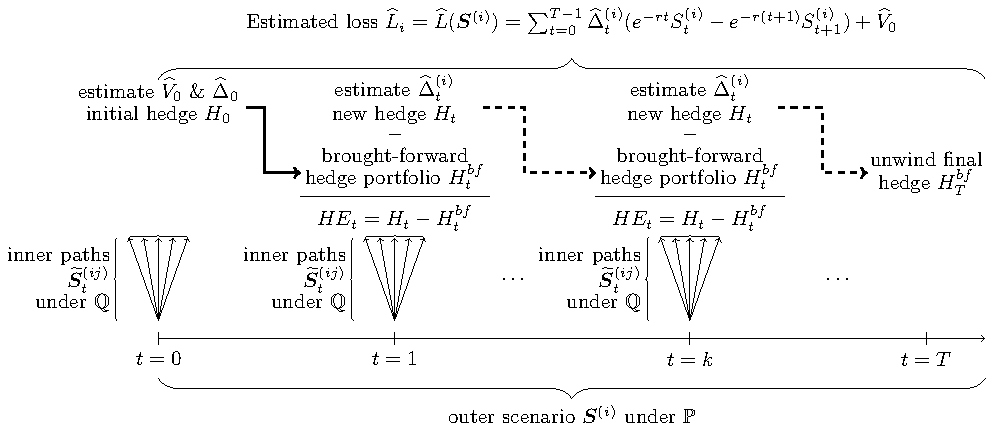
\includegraphics[width=0.85\textwidth]{./project2/figures/sns.pdf}
    \caption{Illustration of multi-period nested simulation that estimates the P\&L for one outer scenario.}
    \label{fig2:illustration}
\end{figure}

Insurers commonly use dynamic hedging to mitigate a market risk exposure in VA contract's embedded options.
In a dynamic hedging program, a hedge portfolio is set up and periodically rebalanced for a portfolio of VA contracts using stocks, bonds, futures, and other derivatives.
For simplicity, in this study we consider delta hedging for a generic VA liability using one stock and one bond.
The metamodeling procedures in Section~\ref{sec2:metamodel2Stage} and Section~\ref{sec2:metamodel1Stage} can be trivially adapted to more general hedging strategies.

Consider a VA contract whose delta hedge portfolio at any time~$t$, $t=0,1,\ldots,T-1$, consists of $\Delta_t$ units in the underlying stock and $B_t$ amount of a risk-free zero-coupon bond maturing at time $T$.
The value of the hedge portfolio at time~$(t-1)$ is:
\begin{equation*}
    H_{t-1} = \Delta_{t-1} S_{t-1} + B_{t-1},
\end{equation*}
where $S_t$ is the underlying stock price and any time $t>0$.
This hedge portfolio is brought forward to the next rebalancing time~$t$, when its value becomes:
\begin{equation*}
    H_{t}^{bf} = \Delta_{t-1} S_{t} + B_{t-1}e^{r}.
\end{equation*}
Therefore, the time~$t$ hedging error, i.e., the cash flow incurred by the insurer due to rebalancing at time~$t$, is
\begin{equation}\label{eq2:hedgingerror}
    HE_t = H_t - H^{bf}_t, \quad t=1,\ldots, T-1.
\end{equation}
The P\&L of the VA contract includes the cost of the initial hedge ($H_0$), the hedging errors~\eqref{eq2:hedgingerror}, the unwinding of the hedge at maturity ($H^{bf}_T$), and the unhedged liability ($V_0$).
Mathematically, the present value of these cash flows is given by
\begin{equation}\label{eq2:lossrv}
L = H_0 + \sum_{t=1}^{T-1} e^{-rt} HE_t - e^{-rT} H^{bf}_T + V_0 = \sum_{t=0}^{T-1}\Delta_t (e^{-rt}S_t - e^{-r(t+1)}S_{t+1}) + V_0,
\end{equation}
where the second equality holds by a telescopic sum simplification of $e^{-rt}B_t$, $t=0,\ldots,T-1$.

In~\eqref{eq2:lossrv}, $\Delta_t$ and $V_0$ are determined by using a risk-neutral measure $\mathbb{Q}$ while the distribution of $L$ is under a real-world measure $\mathbb{P}$.
If $\Delta_t$ and $V_0$ cannot be calculated analytically, a nested simulation is required to estimate the tail risk measure of $L$.
Recall from Section~\ref{subsec:VApayout} that the stock sample path, regardless of the inner or outer simulation or a combination of both, determines the evolution of the triplet $(S_t,F_t,G_t)$.
Specifically, the outer scenarios $\bS^{(i)} = (S_{1}^{(i)},\ldots,S_{T}^{(i)})$, $i=1,\ldots,M$ are generated under $\mathbb{P}$.
At each time~$t=1,\ldots,T-1$ of a given outer scenario $\bS^{(i)}$, inner sample paths $\bStilde_{t}^{(j)} = (\Stilde_{t+1}^{(j)},\ldots,\Stilde_{T}^{(j)})$, $j=1,\ldots,N$ are generated under $\mathbb{Q}$ to estimate $\Delta_t^{(i)}$, $i=1,\ldots,M$.
Also, $V_0^{(i)}$, $i=1,\ldots,M$ are estimated under $\mathbb{Q}$ via inner simulations at time $0$.
Recall from Section~\ref{subsec:VApayout} that the stock's sample path, regardless of inner or outer simulation or a combination of both, determines the evolution of the triplet $(S_t,F_t,G_t)$.
For GMWB, a standard nested simulation procedure to estimate the $\alpha$-CVaR of $L$ is described in Algorithm~\ref{alg2:standardProcedure}.

% For example, for GMWB, a standard nested simulation procedure to estimate the $\alpha$-CVaR of $L$ is as follows:
% \begin{enumerate}
%     \item For $i=1,\ldots,M$, simulate outer scenarios $\bS^{(i)} = (S_{1}^{(i)},\ldots,S_{T}^{(i)})$ under the real-world measure $\mathbb{P}$.
%     Figure~\ref{fig2:illustration} illustrates the inner simulation experiments needed for an outer scenario.
    
%     \item For $t=0$, simulate time-$0$ inner paths $\bStilde_{0}^{(j)} = (\Stilde_{1}^{(j)},\Stilde_{2}^{(j)},\ldots,\Stilde_{T}^{(j)})$, $j=1,\ldots,N$ under $\mathbb{Q}$ {and} then estimate $V_0$ by $\Vhat_0 = \sum_{s=1}^{T} e^{-r(T-s)} [(I_s - F_s)^+- \eta_n F_s]$ and estimate $\Deltahat_0 = \Delta_0(\Stilde_{1}^{(j)},\ldots,\Stilde_{T}^{(j)} | S_0)$ based on~\eqref{eq2:delta}.
%     Note that $S_0$ is known, so these inner paths do not depend on any outer scenario.
%     The same $\Vhat_0$ and $\Deltahat_0$ are used in all scenarios.
    
%     \item Given each scenario $\bS^{(i)}$, the following inner simulation is needed to estimate the corresponding loss $\Lhat_i$ for that scenario.
%     \begin{enumerate}
%         \item At each time~$t=1,\ldots,T-1$, simulate inner paths $\bStilde_{t}^{(ij)} = (\Stilde_{t+1}^{(ij)},\ldots,\Stilde_{T}^{(ij)})$, $j=1,\ldots,N$ under $\mathbb{Q}$ {and} then estimate $\Delta_t$ by $\Deltahat_t^{(i)} = \Delta_t(\Stilde_{t+1}^{(ij)},\ldots,\Stilde_{T}^{(ij)} | \bm{S}_t^{(i)})$ based on~\eqref{eq2:delta}.

%         \item Use scenarios $\bS^{(i)}$ and $\Vhat_0$ and $\Deltahat_t^{(i)}$ to calculate losses $\Lhat_i^{MC}$, $t=0,\ldots,T-1$, based on~\eqref{eq2:lossrv}. Then sort them as $\Lhat^{MC}_{(1)}\leq \Lhat^{MC}_{(2)} \leq \cdots\leq \Lhat^{MC}_{(M)}$.
%     \end{enumerate}

%     \item Estimate $\alpha$-CVaR of $L$ by $\widehat{\CVaR}^{MC}_\alpha = \frac{1}{(1-\alpha)M} \sum_{i=\alpha M + 1}^{M}\Lhat_{(i)}^{MC} = \frac{1}{(1-\alpha)M} \sum_{i \in \widehat{\tail}_{(1-\alpha )M}^{MC}}\Lhat_{i}^{MC}$
%     where $\widehat{\tail}_{k}^{MC}$ denotes a \textit{Monte Carlo tail scenario set} associated with the largest $k$ estimated losses.
% \end{enumerate}

\begin{algorithm} 
\caption{Standard Nested Simulation Procedure for Estimating CVaR for GMWB Hedging Losses}
\begin{algorithmic}[1] \label{alg2:standardProcedure}
    \STATE  For $i=1,\ldots,M$, simulate outer scenarios $\bS^{(i)} = (S_{1}^{(i)},\ldots,S_{T}^{(i)})$ under the real-world measure $\mathbb{P}$.
    \STATE  For $t=0$, simulate time-$0$ inner paths $\bStilde_{0}^{(j)} = (\Stilde_{1}^{(j)},\Stilde_{2}^{(j)},\ldots,\Stilde_{T}^{(j)})$, $j=1,\ldots,N$ under $\mathbb{Q}$, then estimate $V_0$ by $\Vhat_0 = \sum_{s=1}^{T} e^{-r(T-s)} [(I_s - F_s)^+- \eta_n F_s]$ and $\Deltahat_0 = \Delta_0(\Stilde_{1}^{(j)},\ldots,\Stilde_{T}^{(j)} | S_0)$.
    \STATE  Given each scenario $\bS^{(i)}$:
    \begin{enumerate}[label=\alph*., itemsep=0pt, parsep=0pt, topsep=0pt]
        \item   At each time~$t=1,\ldots,T-1$, simulate inner paths $\bStilde_{t}^{(ij)} = (\Stilde_{t+1}^{(ij)},\ldots,\Stilde_{T}^{(ij)})$, $j=1,\ldots,N$ under $\mathbb{Q}$, then estimate $\Delta_t$ by $\Deltahat_t^{(i)} = \Delta_t(\Stilde_{t+1}^{(ij)},\ldots,\Stilde_{T}^{(ij)} | \bm{S}_t^{(i)})$.
        \item   Use scenarios $\bS^{(i)}$ and $\Vhat_0$ and $\Deltahat_t^{(i)}$ to calculate losses $\Lhat_i^{MC}$, $t=0,\ldots,T-1$, then sort them as $\Lhat^{MC}_{(1)}\leq \Lhat^{MC}_{(2)} \leq \cdots\leq \Lhat^{MC}_{(M)}$.
    \end{enumerate}
    \STATE  Estimate $\alpha$-CVaR of $L$ by $\widehat{\CVaR}^{MC}_\alpha = \frac{1}{(1-\alpha)M} \sum_{i=\alpha M + 1}^{M}\Lhat_{(i)}^{MC} = \frac{1}{(1-\alpha)M} \sum_{i \in \widehat{\tail}_{(1-\alpha )M}^{MC}}\Lhat_{i}^{MC}$.
\end{algorithmic}
\end{algorithm}

We refer to the collection of experiments needed conditional on one scenario $\bS^{(i)}$ to estimate $L_i$, that is, all upward arrows in Figure~\ref{fig2:illustration}, as one inner simulation experiment.
We make four observations:
\begin{itemize}
    \item   each inner simulation is time-consuming, as it includes $T$ simulation experiments, one at each time $t=0,\ldots,T-1$,
    \item   after running inner simulations for $M$ scenarios, we obtain simulated data, that is, feature-label pairs, $(\bS^{(i)}, \Lhat_i)$, $i=1,\ldots,M$; the feature vector $\bS$ is $T$ dimensional,
    \item   $\Lhat_i^{MC}$ is a standard Monte Carlo estimator of the true loss for scenario $\bS^{(i)}$. It is an unbiased estimator and its variance is inversely proportional to the number of inner replications $N$. 
    As $N$ approaches infinity, $\Lhat_i^{MC}$ converges to the true loss $L_i$, and
    \item   most importantly, when estimating tail risk measures such as $\alpha$-CVaR, only a small number of estimated losses, that is, those associated with the set of tail scenarios $\widehat{\tail}_{k}$ are used in the estimator.
\end{itemize}

\section{Two-Stage Nested Simulation with Metamodels} \label{sec2:metamodel2Stage}

Based on the three observations above and inspired by~\cite{dang2020efficient}, we propose a two-stage nested simulation procedure which uses a deep neural network metamodel to identify potential tail scenarios.
We present our proposed procedure as a competitor to the standard procedure with $M$ outer scenarios and $N$ inner replications for each outer scenario, as described in Section~\ref{subsec:dynamicHedge}.
We propose a two-stage procedure with a neural network metamodel that aims to produce a CVaR estimate that's as accurate as that of the standard procedure, but uses fewer computations as than latter.

% \begin{itemize}
%     \item[I.] \textbf{Train a neural network metamodel using simulation data.}
%     \begin{itemize}[leftmargin=0pt]
%         \item Use a fraction of the total simulation budget to run Steps 1, 2, and 3 in the standard procedure with the same number of outer scenarios, $M$, but a much smaller number of inner replications, i.e., $N'\ll N$, in each scenario.
%         Then obtain $M$ simulated samples, i.e., feature-label pairs, $(\bS^{(i)}, \Lhat_i)$, $i=1,\ldots,M$.
%         Note that $N'$ may be 10 times or even 100 times smaller than $N$, so the loss estimates $\Lhat_i$ are expected to have larger variance, i.e., more noisy, than the standard procedure's loss estimates.
    
%         \item Use the simulated data, $(\bS^{(i)}, \Lhat_i)$, $i=1,\ldots,M$ to train a neural network.
%         We refer to the trained model as a \textit{metamodel} as denote it by $\Lhat^{PD}(\bS)$.
%         Denote the predicted losses for the outer scenarios by $\Lhat^{PD}_i = \Lhat^{PD}(\bS^{(i)})$, $i=1,\ldots,M$.
    
%         \item Sort the predicted losses $\Lhat^{PD}_{(1)}\leq \Lhat^{PD}_{(2)} \leq \cdots\leq \Lhat^{PD}_{(M)}$ to identify a \textit{predicted tail scenario set} associated with the largest predicted losses, i.e., $\widehat{\tail}_{m}^{PD}:=\{i: \Lhat^{PD}_i > \Lhat^{PD}_{(M-m)}\}$.
%         The number of predicted tail scenarios, $m$, is a user's choice and will be discussed later.
%     \end{itemize}
%         \item[II.] \textbf{Concentrate simulation on predicted tail scenarios.}
%         \begin{itemize}[leftmargin=0pt]
        
%         \item Run Steps 2 and 3 of the standard procedure with the same number of inner replications, $N$, but only on the predicted tail scenarios, i.e., scenarios associated with $\widehat{\tail}_{m}^{PD}$.
%         Denote the standard procedure's estimated losses and sorted losses by $\Lhat^{ML}_i$ and $\Lhat^{ML}_{(i)}$, respectively, $i=1,\ldots,m$.
        
%         \item Estimate the $\alpha$-CVaR of $L$ by $\widehat{\CVaR}^{ML}_\alpha = \frac{1}{(1-\alpha)M} \sum_{i=\alpha M + 1}^{M}\Lhat_{(i)}^{ML} = \frac{1}{(1-\alpha)M} \sum_{i \in \widehat{\tail}_{(1-\alpha )M}^{ML}}\Lhat_{i}^{ML}$
%         where $\widehat{\tail}_{k}^{ML}$ denotes a \textit{predicted tail scenario set} associated with the largest $k$ estimated losses.
%     \end{itemize}
%     \end{itemize}

\begin{algorithm}
\caption{Two-Stage Metamodeling Nested Simulation Procedure for Estimating CVaR}
\begin{algorithmic}[1] \label{alg2:twoStageProcedure}
    \STATE \textbf{Train a neural network metamodel using simulation data:}
    \begin{enumerate} [label=\alph*., itemsep=0pt, parsep=0pt, topsep=0pt]
        \item Use a fraction of the total simulation budget to run Steps 1, 2, and 3 in the standard procedure, i.e., Algorithm~\ref{alg2:standardProcedure}, with the same number of outer scenarios, $M$, but a much smaller number of inner replications, $N' \ll N$, in each scenario. Obtain $M$ simulated samples (feature-label pairs), $(\bS^{(i)}, \Lhat_i)$, $i=1,\ldots,M$. Note that $N'$ may be much smaller than $N$, so $\Lhat_i$ are expected to have larger variance.
        \item Use the simulated data, $(\bS^{(i)}, \Lhat_i)$, $i=1,\ldots,M$ to train a neural network. Refer to the trained model as a metamodel and denote it by $\Lhat^{PD}(\bS)$. Denote the predicted losses for the outer scenarios by $\Lhat^{PD}_i = \Lhat^{PD}(\bS^{(i)})$, $i=1,\ldots,M$.
        \item Sort the predicted losses $\Lhat^{PD}_{(1)}\leq \Lhat^{PD}_{(2)} \leq \cdots\leq \Lhat^{PD}_{(M)}$ to identify a predicted tail scenario set, $\widehat{\tail}_{m}^{PD}$, associated with the largest predicted losses. The number of predicted tail scenarios, $m$, is a user's choice.
    \end{enumerate}
    \STATE \textbf{Concentrate simulation on predicted tail scenarios:}
    \begin{enumerate} [label=\alph*., itemsep=0pt, parsep=0pt, topsep=0pt]
        \item Run Steps 2 and 3 of Algorithm~\ref{alg2:standardProcedure} with the same number of inner replications, $N$, but only on the predicted tail scenarios, i.e., scenarios in $\widehat{\tail}_{m}^{PD}$. Denote the standard procedure's estimated losses and sorted losses by $\Lhat^{ML}_i$ and $\Lhat^{ML}_{(i)}$, respectively, $i=1,\ldots,m$.
        \item Estimate the $\alpha$-CVaR of $L$ by 
        $$\widehat{\CVaR}^{ML}_\alpha = \frac{1}{(1-\alpha)M} \sum_{i=\alpha M + 1}^{M}\Lhat_{(i)}^{ML} = \frac{1}{(1-\alpha)M} \sum_{i \in \widehat{\tail}_{(1-\alpha )M}^{ML}}\Lhat_{i}^{ML},$$ 
        where $\widehat{\tail}_{k}^{ML}$ denotes a predicted tail scenario set associated with the largest $k$ estimated losses.
    \end{enumerate}
\end{algorithmic}
\end{algorithm}

Similar to~\cite{dang2020efficient}, the proposed two-stage procedure in Algorithm ~\ref{alg2:twoStageProcedure} uses the metamodel predictions to identify the predicted tail scenario set in Stage 1.
However, different from their fixed-budget simulation design, we attempt to achieve a target accuracy.
Specifically, in Stage 2 we propose using a standard procedure with the same number of inner replications, $N$, as a competing simulation procedure (or a benchmark).
There are two different experiment designs for nested simulation procedures: fixed-budget design and fixed-accuracy design.
In a fixed-budget design, the simulation budget is fixed and the goal is to achieve the highest accuracy possible within the budget.
Let $\Gamma = MN$ be the simulation budget for the standard procedure, where each scenario receives $\frac{\Gamma}{M}$ inner replications.
In the proposed two-stage procedure, suppose Stage 2 uses 1\% of the simulation budget, $\alpha = 95\%$, and $m=(1-\alpha)M$, then $99\%$ of the simulation budget is concentrated on $5\% M$ predicted tail scenarios in Stage 2.
In other words, each predicted tail scenario receives $\frac{99\% \Gamma}{5\% M}$ inner replications, almost 20 times more than that in the standard procedure.
This budget concentration is expected to improve the estimation accuracy of the two-stage procedure compared to a standard procedure with the same budget. 
If the metamodel is accurate in predicting true tail scenarios, then the two-stage procedure is expected to achieve higher accuracy than the standard procedure with the same budget.
However, we believe that the goal of designing an efficient simulation procedure is to solve practical problems faster, so a target-accuracy design is more suitable, which refers to obtaining a similar level of accuracy as the standard procedure but with much less simulation budget.
One other reason for this fixed-accuracy design is to investigate whether deep neural network metamodels trained with much noisier labels can identify true tail scenarios with similar accuracy as the standard procedure.
The size of the predicted tail scenario set in Stage 1, $m$, is an important experiment design parameter that affects the correct identification of true tail scenarios and ultimately affects the estimation accuracy for CVaR.
Clearly, there is a lower bound $m \geq (1-\alpha)M$ because the $\alpha$-CVaR is estimated by the average of $(1-\alpha)M$ largest losses at the end of Stage 2.
For ease of reference, we call the additional percentage of predicted tail scenarios above this lower bound, i.e., $\epsilon = \frac{m - (1-\alpha)M}{M}$, as a \textit{safety margin}.
On one hand, large $\epsilon$ is not desirable because it increases computations in Stage 2.
On the other hand, $\epsilon$ should be set reasonably large so more true tail scenarios are included in the the predicted tail scenario set $\widehat{\tail}_{m}^{PD}$ and are ultimately included in $\widehat{\tail}_{(1-\alpha )M}$ at the end of Stage 2.
The selection of $m$ is highly dependent on the choice of the metamodel.
Due to the simulation errors and approximation error in the metamodel in Stage 1, we do not expect perfect match between the true tail scenario set $\tail_{k}$ and the predicted tail scenario set $\widehat{\tail}_{k}^{PD}$ for any size $k$.
This means that we should not set $m$ at its lower bound: Some safety margin $\epsilon M$ should be added to the predicted tail scenario set, i.e., $m = (1-\alpha )M + \epsilon M$, to increase the likelihood that $\tail_{k} \subseteq \widehat{\tail}_{m}^{PD}$ and that the true tail scenarios are included in estimating $\alpha$-CVaR at the end of Stage 2.
The choice of safety margin $\epsilon$ is not trivial, and it should be set based on the metamodel's accuracy in identifying true tail scenarios.
In the numerical experiments, we examine the relationship between the safety margin and the correct identification of true tail scenarios for different metamodels.

\section{Single-Stage Nested Simulation with Neural Network Metamodels} \label{sec2:metamodel1Stage}

In our exploratory experiment with the two-stage procedure, we observe that a suitable metamodel trained with noisy labels is accurate enough to identify true tail scenarios with a relatively small safety margin.
This observation motivates us to propose a single-stage procedure that uses the identical neural network metamodel, not for the purpose of differentiating between tail and non-tail scenarios, but rater to estimate the CVaR directly using the predicted losses. 

\begin{algorithm}
\caption{Single-Stage Metamodeling Nested Simulation Procedure for Estimating CVaR}
\begin{algorithmic}[1] \label{alg2:oneStageProcedure}
    \STATE Run Step 1 of Algorithm~\ref{alg2:twoStageProcedure}, and denote the predicted losses by
    $\Lhat^{PD}_i = \Lhat^{PD}(\bS^{(i)})$, $i=1,\ldots,M$.
    \STATE Sort the predicted losses $\Lhat^{PD}_{(1)}\leq \Lhat^{PD}_{(2)} \leq \cdots\leq \Lhat^{PD}_{(M)}$ to identify the largest predicted losses. 
    \STATE Directly estimate the risk measure (e.g., $\alpha$-CVaR) of $L$ using the metamodel predictions: Calculate $\widehat{\CVaR}^{PD}_\alpha = \frac{1}{(1-\alpha)M} \sum_{i=\alpha M + 1}^{M}\Lhat^{PD}_{(i)}$.
\end{algorithmic}
\end{algorithm}

The single-stage procedure has three major advantages over the two-stage procedure:
(1) the single-stage procedure is expected to be more efficient than the two-stage procedure because it does not require the running the standard procedure in Stage 2, 
(2) the safety margin $\epsilon$ is not needed in the single-stage procedure, and
(3) most importantly, the single-stage procedure is not limited to just estimating tail risk measures and can be extended to provide a broader assessment of risk. 
It can be naturally adapted to estimate risk measures that require the knowing of the entire loss distribution, such as the standard deviation or the squared tracking error.
In our numerical experiments, we will compare the single-stage procedure to the two-stage procedure and the standard procedure in estimating the $\alpha$-CVaR of the hedging losses for GMWB, and we will also examine the single-stage procedure's performance in estimating the standard deviation of the hedging losses.


\section{Numerical Results} \label{sec2:numerical}

We conduct a series of simulation experiments to (1) demonstrate the efficiency of the proposed metamodeling procedures and (2) examine the error tolerance to noisy training data in deep learning models.
The problem settings in our experiments are identical to those in~\cite{dang2020efficient}:
we consider estimating the $95\%$ CVaR of the hedging loss of a GMWB contract, which is one of the most complex VA contracts in the market.
The VA contracts have a 20-year maturity and are delta-hedged with monthly rebalancing, i.e., $T=240$ rebalancing periods.
The gross and net management fees are $\eta_g = 0.2\%$ and $\eta_n=0.1\%$, respectively.
The withdrawal rate for GMWB is $0.375\%$ per month.
% To make our examples more realistic, the VAs are also subject to dynamic lapse as specified in Section~4.3 of~\cite{dang2020efficient}.
The risk-free rate is 0.2\% per period and the underlying asset $S_t$ is modeled by a regime-switching geometric Brownian motion with parameters specified in Table~2 of~\cite{dang2020efficient}.

To compare the numerical performances of different simulation procedures, we create a benchmark dataset with a large-scale nested simulation: We first simulate $M=\num{100000}$ outer scenarios, i.e., $240$-periods stock paths $\bS^{(1)},\ldots,\bS^{(M)}$ under $\mathbb{P}$ and used these outer scenarios in all further experiments.
Note that the 5\% tail scenario set includes $5\!,\!000$ scenarios.
As the hedging losses for these scenarios cannot be calculated analytically, we run inner simulations with a large number of replications, $N=\num{100000}$, conditional on each of the $M$ scenarios.
We denote these losses by $L_1,\ldots,L_M$ and will refer to them as \textit{true losses}.
We also use these true losses to estimate $\widehat{\CVaR}_{95\%}$ and denote the corresponding \textit{true tail scenario set} by $\tail_{5000}$.
Lastly, we refer to the set of feature-label pairs $\{(\bS^{(i)}, L_i): i=1,\ldots,M\}$ as a \textit{true dataset}.
Note that the feature vector $\bS$ is a 240-dimension stock path.

We compare our two-stage procedure to a standard nested simulation procedure that runs $N=\num{1000}$ inner replications for each of the $M=\num{100000}$ outer scenarios.
In Stage 1 of the proposed procedure, we first run inner simulations with $N'=100$ inner replications for each of the $M=\num{100000}$ outer scenarios.
So, Stage 1's simulation budget is $10\%$ of the standard procedure's.
The resulting feature-label pairs $\{(\bS^{(i)}, \Lhat_i): i=1,\ldots,M\}$ is used for training different  metamodels.
Specifically, following the convention in machine learning research, we split this dataset into three parts: The training, validation, and test sets have $90\!,\!000$, $5\!,\!000$, and $5\!,\!000$ data points (90\%, 5\%, and 5\% of the dataset), respectively.
At the end of Stage 1, $m$ predicted tail scenarios, are identified by the trained metamodels.
In Stage 2, $N=\num{1000}$ inner replications are run for all predicted tail scenarios.
Stage 2's simulation budget is $\frac{m}{M}$ of the standard procedure's.
In short, the two-stage procedure uses $15\% - 30\%$ of the standard procedure's budget for a safety margin between $0\% - 15\%$.

Five metamodels are considered in this experiment: multiple linear regression (MLR), quadratic polynomial regression (QPR) without interaction terms, feed-forward neural network (FNN), recurrent neural network (RNN), and long short-term memory (LSTM) network.
MLR and QPR are considered as extensions of regression metamodels in the nested simulation literature.
FNN is a generic neural network while RNN and LSTM are specialized models to accommodate the sequential structure of our time-series features.
A $\tanh$ activation function is used for RNN and LSTM layers, and a Rectified Linear Unit (ReLU) activation function is used for the fully-connected layers.
All neural network metamodels are trained by the Adam optimizer~\citep{kingma2014adam} with an initial learning rate of $0.001$ and an exponential learning rate decay schedule.
FNN is trained with a dropout rate of 20\%.
RNN and LSTM are trained with a dropout rate of 10\%.
The architectures and training settings are typical choices in the deep learning literature.
The training labels are normalized to have zero mean and unit standard deviation.
The architectures and the numbers of trainable parameters are shown in the first two columns of Table~\ref{tab:gmwb_arch}.
We see that the three deep neural network metamodels' have orders of magnitudes more trainable parameters than the two regression models.
In machine-learning terminologies, the three deep neural network models have much higher \textit{model capacities}.

\begin{table}[ht!]
    \centering
    \footnotesize
    \begin{tabular}{lccccc}
    \toprule
    \textbf{Model} & \textbf{\makecell{Layer size}} & \textbf{\makecell{Capacity}} & \textbf{Training error} & \textbf{Test error} & \textbf{True error}\\
    \midrule
    MLR & N/A & $241$ & $0.707 (\pm 3.6 \times 10^{-4})$ & $0.877 (\pm 0.001)$ & $0.694 (\pm 0.000)$ \\
    QPR & N/A & $481$ & $0.544 (\pm 0.000)$ & $0.636 (\pm 0.001)$ & $0.531 (\pm 0.000)$ \\
    FNN & $240, 128, 16$ & $35\!,\!009$ & $0.118 (\pm 0.001)$ & $0.247 (\pm 0.002)$ & $0.113 (\pm 0.001)$ \\
    RNN & $(240, 32), (240, 4), 32$ & $32\!,\!021$ & $0.132 (\pm 0.008)$ & $0.137 (\pm 0.008)$ & $0.119 (\pm 0.008)$ \\
    LSTM & $(240, 32), (240, 4), 32$ & $35\!,\!729$ & $0.075 (\pm 0.004)$ & $0.079 (\pm 0.005)$ & $0.063 (\pm 0.004)$ \\
    RNN$^*$\footnotemark & $(240, 32), (240, 4), 32$ & $32\!,\!021$ & $0.109 (\pm 0.005)$ & $0.128 (\pm 0.005)$ & $0.109 (\pm 0.005)$ \\
    \bottomrule
    \end{tabular}
    \caption{Architectures and MSEs of metamodels for GMWB inner simulation model.}
    \label{tab:gmwb_arch}
\end{table}

\footnotetext{Results of the well-trained RNN, where the ones suffers from the vanishing gradient issue are removed from the averages.}

For each metamodel, 50 independent macro replications are run\footnote{Each macro replication includes simulating a noisy dataset, separating it into training and test data, fitting a metamodel, and making predictions}.
The last three columns in Table~\ref{tab:gmwb_arch} display the average squared errors between the predicted losses and the losses (labels) in different datasets.
The half lengths of their 95\% confidence interval of these quantities are also reported in parentheses.
We first observe that the two regression metamodels' errors are larger than those of three deep neural network models.
This is because model capacities of the regression metamodels are too low to learn the complex dynamic hedging simulation model.
All neural network metamodels have high model capcities comparing with the number of data points in the training set, i.e., $90\!,\!000$.
This is not a huge concern for the deep neural networks.
In neural network literature, the number of trainable parameters is often much larger than the number of data points in the training set.
AlexNet~\citep{krizhevsky2012imagenet}, a well-known convolutional neural network, has 60 million parameters and is trained on the ImageNet dataset with 1.2 million images.
Other examples include generative pre-trained transformer models like BERT~\citep{devlin2018bert} and GPT-3~\citep{brown2020language}, which have billions of parameters and are trained on large-scale text corpora.
The reason for not overfitting is still an open question in deep learning research.
One possible explanation is that the optimization surface of deep neural networks is highly non-convex and has many local minima.
As a result, given a good initialization, the optimization algorithm is likely to find a solution that generalizes well to unseen data.

There are also differences among the three deep neural network models due to having different architectures.
The FNN is a generic neural network, its test error is larger than the training error, which is a sign of over-fitting and poor generalization.
In contrast, RNN and LSTM networks have recurrent strucutures and are designed to capture temporal relationship in the high-dimensional feature.
As a result, they have lower training errors, i.e., they fit the data better, and have lower testing error, i.e., they generalize better.
Notably, the true errors for the deep neural network metamodels are lower than the test errors.
This is a sign of the metamodels' ability to learn the true feature-label relationship with noisy training labels. 
Section~\ref{subsec2:noiseTolerance} investigates this phenomenon in more details.

Comparing the two metamodels with recurrent structures, A LSTM network overcomes two key drawbacks of a crude RNN.
\begin{enumerate}
    \item It avoids the vanishing gradient problem during training, which makes the LSTM easier to than the RNN. Figure~\ref{fig2:QQ_RNN} shows the quantile-quantile (QQ) plots between the \textbf{training} labels and the RNN predictions for two macro replications, where training of the latter is hindered by the vanishing gradient problem\footnote{A well-trained RNN stops early at around 300 training epochs, while an ill-trained RNN uses up all 1000 training epochs.}. 
    As a result, the half length of the 95\% confidence interval of the RNN's training error is much larger than all other metamodels. The last row of Table~\ref{tab:gmwb_arch} shows the average squared errors of the good RNN metamodels that are successfully trained. 
    Removing the RNN metamodels that are ill-trained, the average squared errors of the RNN metamodels are lower than those of the FNN, but the half lengths of their 95\% confidence intervals are larger than those of the FNN. 
    This suggests that the RNN is more sensitive to noise in stochastic gradient descent than the FNN.
    \item A LSTM introduces three gates that regulate the flow of information. 
    These gates decide what information should be kept or discarded. This makes a LSTM more capcable of learning long-term dependencies. 
    Since the feature in our dynamic hedging problem is a 240-dimensional time series, a LSTM is more suitable than a crude RNN.
    The network architecture serves as a prior knowledge that guides the optimization algorithm to find a solution that generalizes well to unseen data, and it significantly impact the metamodel's performance.
    It is important to choose a suitable architecture with a pre-set capacity that is large enough to learn the true feature-label relationship.
\end{enumerate}


\begin{figure}[ht!]
    \centering
    \begin{subfigure}{0.48\textwidth}
        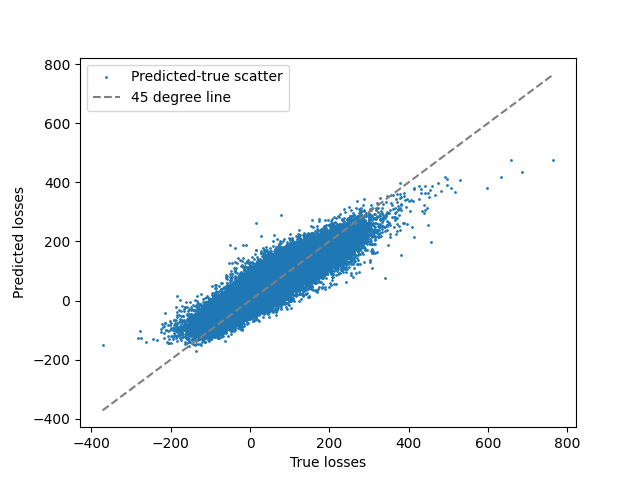
\includegraphics[width=\textwidth]{./project2/figures/qqPlots/rnnGood.png}
        \caption{A good RNN metamodel}
    \end{subfigure}\hfill
    \begin{subfigure}{0.48\textwidth}
        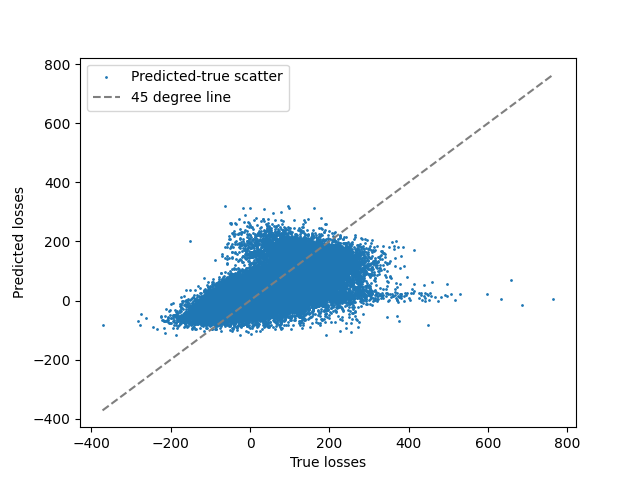
\includegraphics[width=\textwidth]{./project2/figures/qqPlots/rnnBad.png}
        \caption{A bad RNN metamodel}
        \label{subfig2:badRNN}
    \end{subfigure}
    \caption{QQ-plots between true labels (x-axis) and predicted losses (y-axis) for the RNN metamodel.} 
    \label{fig2:QQ_RNN}
\end{figure}

Recall that all three data sets are generated from the same simulation model, but the true data set is less noisy than the training and test data.
Part of the training error is due to simulation noise, and this noise is lower in the true error.
We observe that the two regression metamodels not only generalize to the test data poorly but also generalize to the true data poorly.
In contrast, the deep neural network metamodels generalize better to the true data than to the test data.
Figure~\ref{fig2:QQ_REG} and Figure~\ref{fig2:QQ_NN} shows the QQ plots between the \textbf{true} labels and the predicted losses for the regression metamodels and the neural network metamodels, respectively.

\begin{figure}[ht!]
    \centering
    \begin{subfigure}{0.48\textwidth}
        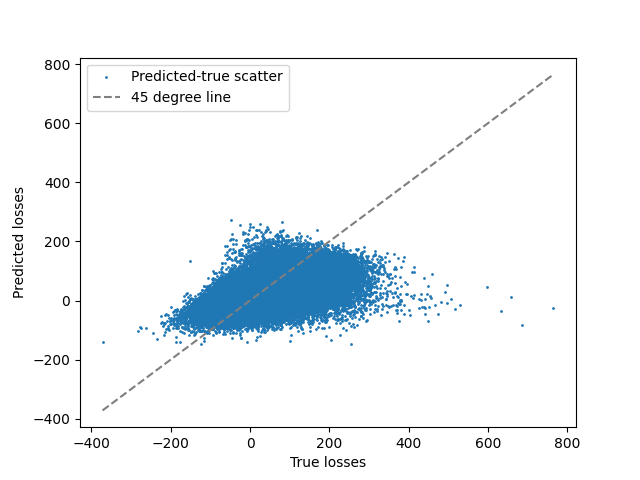
\includegraphics[width=\textwidth]{./project2/figures/qqPlots/mlrLN.png}
        \caption{MLR metamodel}
    \end{subfigure}\hfill
    \begin{subfigure}{0.48\textwidth}
        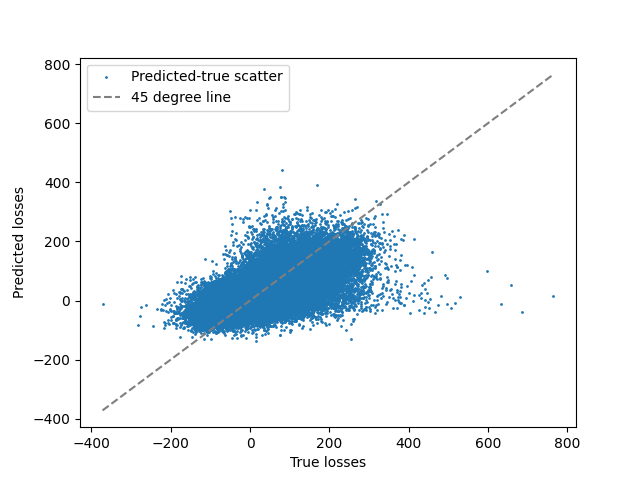
\includegraphics[width=\textwidth]{./project2/figures/qqPlots/qprLN.png}
        \caption{QPR metamodel}
    \end{subfigure}
    \caption{QQ-plots between true losses (x-axis) and predicted losses (y-axis) for regression metamodels.} 
    \label{fig2:QQ_REG}
\end{figure}

Comparing with the MSE table in Table~\ref{tab:gmwb_arch} that summarizes the overall fit, QQ plots offer a closer look at the metamodels' performance on different parts of the loss distribution.
Figure~\ref{fig2:QQ_REG} show that the regression metamodels' predictions are far from the true losses, especially on the tails.
Between the two regression metamodels, the QPR metamodel has a slightly better fit for larger losses.
Nevertheless, both regression metamodels have poor fits to the true data, and their fit on the tail is particularly undesirable.
The poor fit on the tail hinders the regression metamodels' ability to identify true tail scenarios and ultimately leads to poor CVaR estimates.
Adding the quadratic terms, our QPR metamodel is considered as a natural extension of the MLR.
Attempts to further improve the regression metamodels by adding interaction terms or higher-order terms do not improve the fit.
Having 240 features, feature engineering for regression metamodels is not a trivial task and is highly dependent on the simulation model. 
As a result, the regression metamodels are not flexible enough to capture the complex feature-label relationship in the dynamic hedging simulation model.

\begin{figure}[ht!]
    \centering
    \begin{subfigure}{0.48\textwidth}
        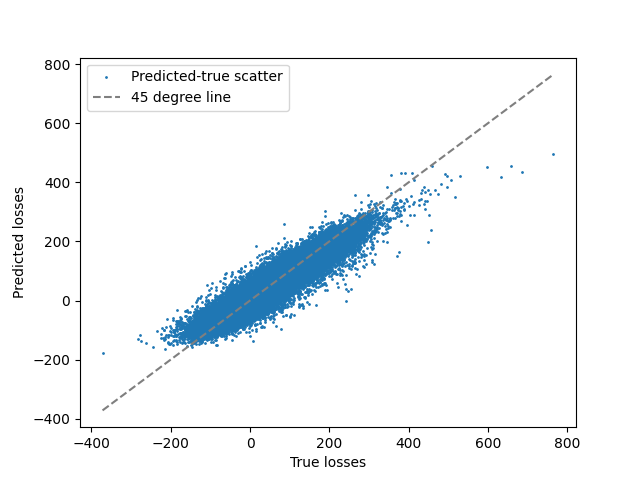
\includegraphics[width=\textwidth]{./project2/figures/qqPlots/fnnLN.png}
        \caption{FNN metamodel}
    \end{subfigure}\hfill
    \begin{subfigure}{0.48\textwidth}
        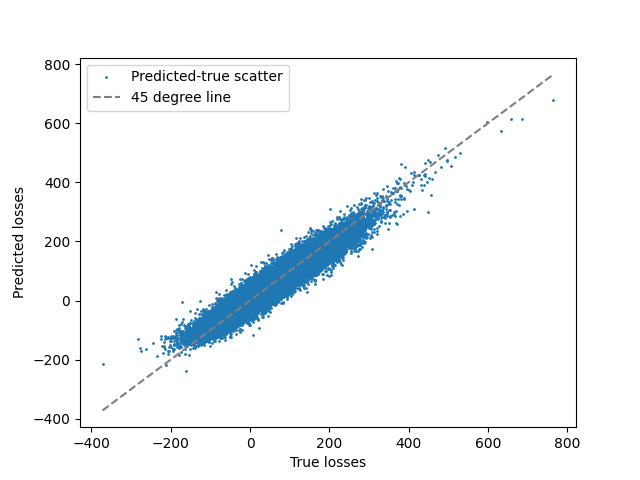
\includegraphics[width=\textwidth]{./project2/figures/qqPlots/lstmLoCapLN.png}
        \caption{LSTM metamodel}
    \end{subfigure}
    \caption{QQ-plots between true losses (x-axis) and predicted losses (y-axis) for neural network metamodels.} 
    \label{fig2:QQ_NN}
\end{figure}

In Figure~\ref{fig2:QQ_NN}, we illustrate the fit of the neural network metamodels.
The FNN has a better fit than the regression metamodels, but it still has a poor fit on the tails.
We observe that the LSTM metamodels' QQ-plots closely follow that 45-degree line.
Again, these metamodels are trained on noisy data, so the good fit to the true data should not be taken for granted.
This implies that these models indeed learn the true feature-label relationship in the dynamic hedging simulation model (i.e., true loss labels) even though they are trained on noisy observations (e.g., training labels) of the model.

From a unique analytical standpoint, our numerical study offers a methodical exploration into the robustness of deep neural network models against noise in training labels. 
By employing the standard nested simulation procedure in Algorithm~\ref{alg2:standardProcedure} as a data generator, we gain the ability to manipulate the noise level through adjusting the number of inner replications while keeping the same simulation procedure.
As a result, this approach provides a controlled environment to examine the impact of label noise on neural network model.
It allows us to generate our true dataset that approximates the true hedging losses with a high degree of precision, and, as a result, it enables us to explore the crucial question of whether deep learning models are capable of learning the true feature-label relationship from noisy training labels.
Our numerical results in Table~\ref{tab:gmwb_arch} and the QQ plots provide direct evidence that deep neural network models are indeed able to cut through the noise in the training labels and learn the true feature-label relationship.
The LSTM metamodels' ability to learn the true feature-label relationship is crucial for the two-stage procedure to identify true tail scenarios and produce accurate CVaR estimates.

\subsection{Two-Stage Procedure} \label{subsec:twoStageProcedure}

In our proposed two-stage procedure, the metamodel is used to identify the predicted tail scenario set, on which the standard nested simulation procedure is run in Stage 2 to estimate the $95\%$-CVaR.
An accurate identification of the true tail scenarios is crucial.
In a two-stage procedure, metamodels' overall prediction errors measured by the MSEs in Table~\ref{tab:gmwb_arch} are not the determining factor, but their ability to effectively rank the scenarios by their \textbf{true} losses is most critical in producing accurate CVaR estimates.

\begin{figure}[ht!]
    \centering
    \begin{subfigure}{0.48\textwidth}
        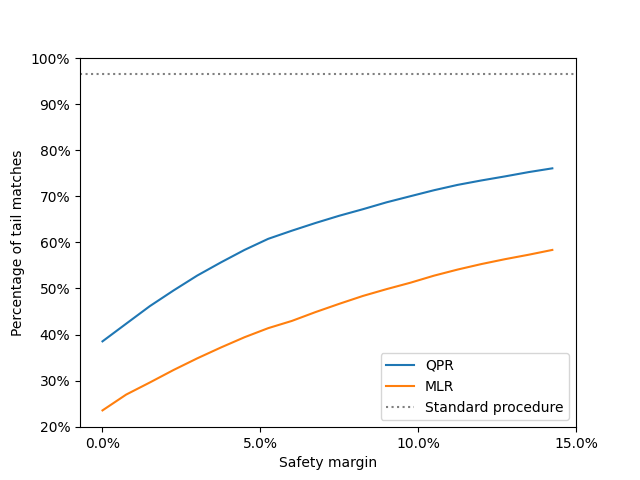
\includegraphics[width=\textwidth]{./project2/figures/tailMatches/regLN.png}
        \caption{Regression metamodels}
    \end{subfigure}\hfill
    \begin{subfigure}{0.48\textwidth}
        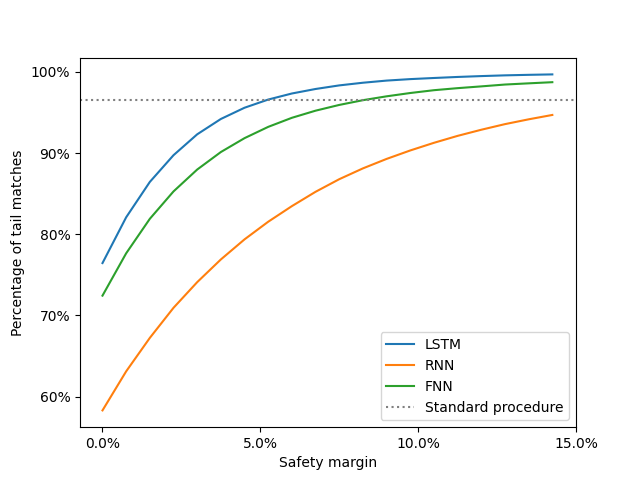
\includegraphics[width=\textwidth]{./project2/figures/tailMatches/nnLN.png}
        \caption{Neural network metamodel}
    \end{subfigure}
    \caption{Percentage of correctly identified true tail scenarios by different metamodels.}
    \label{fig2:tailMatches}
\end{figure}

Figure~\ref{fig2:tailMatches} depicts the average percentage of correctly identified true tail scenarios\footnote{Each quantity is averaged over 50 macro replications.}  by different metamodels for different safety margins.
The percentage of tail matches of the traditional regression metamodels are significantly lower than the ones of the neural networks.
We see that a poor metamodel like the QPR identifies less than 40\% of the true tail scenario without any safety margin.
In contrast, a good metamodel like the LSTM identifies more than 75\% of the true tail scenarios without any safety margin and more than the QPR metamodel does with 15\% of safety margin\footnote{The metamodel in~\cite{dang2020efficient} identifies 100\% of the true tail scenarios on with a 10\% safety margin for a GMAB contract.
The GMAB contract is simpler than the GMWB contract, and the true tail scenarios are easier to identify. 
For a GMAB, our LSTM metamodel identifies 100\% of the true tail scenarios with a 2.5\% safety margin}.
The RNN metamodel suffers from the vanishing gradient problem during training. 
For some macro replications (as shown in Figure~\ref{subfig2:badRNN}), the RNN metamodels' predictions are far from the true losses, especially on the tails.
The FNN metamodel has a better fit than the regression metamodels, but it does not have the same level of accuracy as the LSTM metamodel, which is a specialized network to capture the sequential structure of our time-series features.
For comparison, the horizontal dotted line shows the percentage of correctly identified true tails for the standard nested simulation procedure.
A good metamodel should be able to identify a similar percentage of true tail scenarios as the standard procedure does with a reasonable safety margin.
Otherwise, the two-stage procedure will offer no computational advantage in simulation budget over the standard procedure.
The LSTM metamodel can reaches similar percentage with a 5\% safety margin.
This indicates that the LSTM metamodel should be able to reach the same level of accuracy as the standard procedure with only 20\% of the simulation budget.

\begin{figure}[ht!]
    \centering
    \begin{subfigure}{0.48\textwidth}
        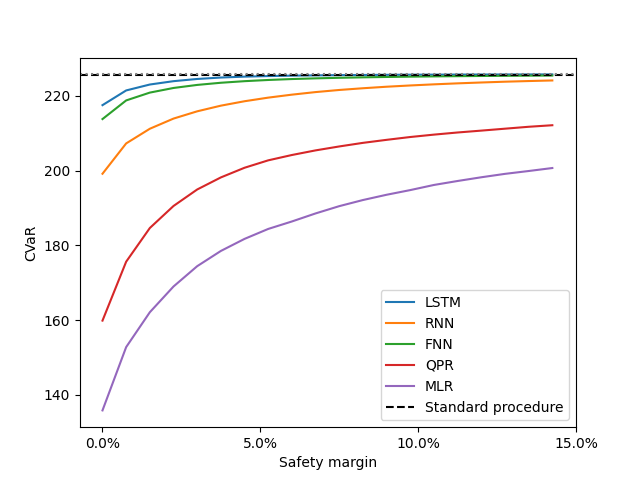
\includegraphics[width=\textwidth]{./project2/figures/CVaR/allLN.png}
        \caption{Safety margin 0\% - 15\%.}
        \label{subfig2:AllSafetyMargin}
    \end{subfigure}
    \begin{subfigure}{0.48\textwidth}
        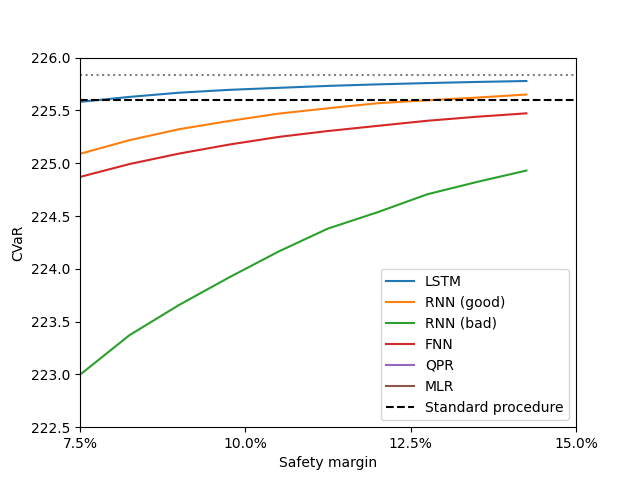
\includegraphics[width=\textwidth]{./project2/figures/CVaR/zoomedLN.png}
        \caption{Safety margin 7.5\% - 15\%.}
        \label{subfig2:ZoomedSafetyMargin}
    \end{subfigure}
    \caption{Average 95\%-CVaR estimates by different procedures. Right figure is a zoomed-in version of left figure.} 
    \label{fig2:CVaR95}
\end{figure}

Lastly, we return to our original goal of estimating the 95\%-CVaR of the dynamic hedging error.
Figure~\ref{fig2:CVaR95} shows the 95\%-CVaR estimates for all five metamodels with different safety margins, averaged over 50 macro replications.
Figure~\ref{subfig2:ZoomedSafetyMargin} is a zoomed version of Figure~\ref{subfig2:AllSafetyMargin}.
Because the safety margin only affects the two-stage procedure, the true 95\%-CVaR and the one estimated by the standard procedure are horizontal (solid and dotted, respectively) lines in Figure~\ref{fig2:CVaR95}.
We observe that, with reasonable safety margins, the two-stage procedures with a LSTM metamodel consistently produce estimates that are as accurate as the standard procedure's estimate.
The amount of computational savings is substantial.
The LSTM is particularly superior to other metamodels as it accurately identifies the true tail scenarios and produces highly accurate CVaR estimates with small safety margins.
By concentrating the simulation budget on the predicted tail scenarios, the two-stage procedure with the LSTM metamodel is able to achieve a similar accuracy as the standard procedure with a much smaller simulation budget.
As the percentage of correctly identified tails approaches 100\%, the two-stage procedure's CVaR estimates does not converge to the true value but to the standard procedure's estimate.
This is because the two-stage procedure's CVaR estimates are based on the standard procedure's estimates on the predicted tail scenarios, and the standard procedure's estimates themselves are also noisy.


\subsection{Noise Tolerance of Deep Neural Network Metamodels} \label{subsec2:noiseTolerance}

For financial and actuarial applications, regulators and practitioners are often concerned about the robustness of deep neural network models to noise in training labels, which hinders the adoption of these models in practice.
Since the true relationship is unknown in real-world applications, most deep learning literature illustrates the impact of noise by artificially injecting noise into real-world datasets, which is already noisy before the injection.
In our numerical experiments, we are able to use Monte Carlo simulation generate a true dataset that approximates the true hedging losses with a high degree of precision, and, as a result, we are able to explore the crucial question of whether deep learning models are capable of learning the true feature-label relationship from noisy training labels.
In this section, we treat the standard nested simulation procedure as a data generator and examine the noise tolerance of LSTM metamodels by varying the numbers of outer scenarios ($M$) and inner replications ($N$) used to generate the training data.
The number of outer scenarios corresponds to the number of feature-label pairs in the training dataset, and the number of inner replications controls the noise level in the training labels.
Recall that we use the standard nested simulation procedure with $N=100$ inner replications in our previous experiments, and we will refer to the resulting training dataset as the \textit{low-noise dataset}.
We also generate a \textit{medium-noise dataset} and a \textit{high-noise dataset} by running the standard nested simulation procedure with $N=10$ and $N=1$ inner replications, respectively.
By altering the data quantity and quality, we conduct a sensitivity analysis on the LSTM metamodels' noise tolerance.
We study the impact of noisy data on two LSTM metamodels with different model capacities, i.e., different numbers of trainable parameters.
The two LSTM metamodels has the same number of layers, but their numbers of hidden units in each layer are different.
More specfically, the high-capacity LSTM metamodel has $128$ and $16$ hidden units in the first and second LSTM layers, respectively, while the low-capacity LSTM metamodel has $32$ and $4$.

The maximum number of data points in the training dataset is set to $M = \num{100000}$.
The training dataset is split into training and test sets with a 90\%-10\% ratio.
The true labels are generated by running the standard nested simulation procedure with $N=\num{100000}$ inner replications for each of the $\num{100000}$ outer scenarios.
The reason for using a maximum of $\num{100000}$ data points is precisely due to the computational cost of running the standard nested simulation procedure.
For consistency, the LSTM metamodels are trained with the same architecture and training settings as in the previous experiments.

\begin{table}[ht!]
    \small
    \centering
    \begin{tabular}{lccccc}
        \toprule
        \textbf{Model}      & \textbf{Noise level}   & \textbf{Training error}   & \textbf{Test error}   & \textbf{True error}\\
        \midrule
        LSTM                & $N=100$                & $0.075 (\pm0.004)$        & $0.079(\pm0.005)$     & $0.063 (\pm0.004)$ \\ 
        High-capacity LSTM  & $N=100$                & $0.068 (\pm0.004)$        & $0.102(\pm0.006)$     & $0.060 (\pm0.004)$ \\
        Difference          & $N=100$                & $-0.007$                  & $0.023$               & $-0.003$ \\
        \hline
        LSTM                & $N=10$                 & $0.195 (\pm0.001)$        & $0.193(\pm0.001)$     & $0.070 (\pm0.001)$ \\
        High-capacity LSTM  & $N=10$                 & $0.157 (\pm0.002)$        & $0.199(\pm0.002)$     & $0.065 (\pm0.001)$ \\
        Difference          & $N=10$                 & $-0.038$                  & $0.006$               & $-0.005$ \\
        \hline
        LSTM                & $N=1$                  & $1.366 (\pm0.006)$        & $0.781(\pm0.005)$     & $0.129 (\pm0.002)$ \\
        High-capacity LSTM  & $N=1$                  & $1.354 (\pm0.006)$        & $0.795(\pm0.005)$     & $0.149 (\pm0.002)$ \\
        Difference          & $N=1$                  & $-0.012$                  & $0.014$               & \textcolor{red}{$0.020$} \\
        \bottomrule
    \end{tabular}
    \caption{MSEs of LSTM metamodels.}
    \label{tab:lstm_arch}
\end{table}

The first two rows of Table~\ref{tab:lstm_arch} shows the average squared errors and the half widths of their 95\% confidence intervals between the metamodel predictions and the labels in the training dataset and the true dataset.
The test errors are included as a practical measure of the metamodels' generalization ability.
For this particular experiment, we are more interested in the true errors, which measure the metamodels' ability to learn the true feature-label relationship from the low-noise, medium-noise, and high-noise datasets.
We first observe that all the true errors are lower than the training errors, indicating that the LSTM metamodels generalize well to predicting the true losses.
Both LSTM metamodels are able to learn the true feature-label relationship from the low-noise and medium-noise datasets.
However, when the noise level is high, both LSTM metamodels have high true error.
The diffences in the errors between the LSTM metamodels are also reported in the last rows of Table~\ref{tab:lstm_arch}.
A positive difference indicates that the high-capacity LSTM has higher errors than the LSTM.
We observe that both LSTM metamodels have similar errors on the low-noise and medium-noise datasets.
However, when the noise level is high, the high-capacity LSTM has higher errors than the regular LSTM.
This is because the high-capacity LSTM has more trainable parameters and is more prone to over-fitting to the noise in the training labels.
In contrast, the LSTM metamodel is more robust to label noise and is able to learn the true feature-label relationship better from the high-noise dataset.
In practice, since the true relationship is unknown, the true error is not readily available.
The test error approximates the true error and is directly observable.
The difference in test errors of the LSTM metamodels are inconsistent with the differences in true errors.
Therefore, test errors are not reliable indicators of the metamodels' noise tolerance.
For practical applications that utilize nerual networks as metamodels, we recommend not simulating the test scenarios.
Instead, we recommend simulating the true contract losses on a few tail and non-tail training scenarios to evaluate the metamodels' noise tolerance.

In summary, our numerical experiments demonstrate that both LSTM metamodels are capable of learning the true inner simulation model from noisy training labels.
In most cases, a high-capacity metamodel is better.
Nevertheless, in extreme circumstances when the noise level is too high, using a high capacity metamodel leads to severe overfitting and poor generalization.
Hence, domain knowledge about the right architecture for the task and knowledge about the noise level in the training labels are beneficial for choosing the right metamodel.

\begin{figure}[ht!]
    \centering
    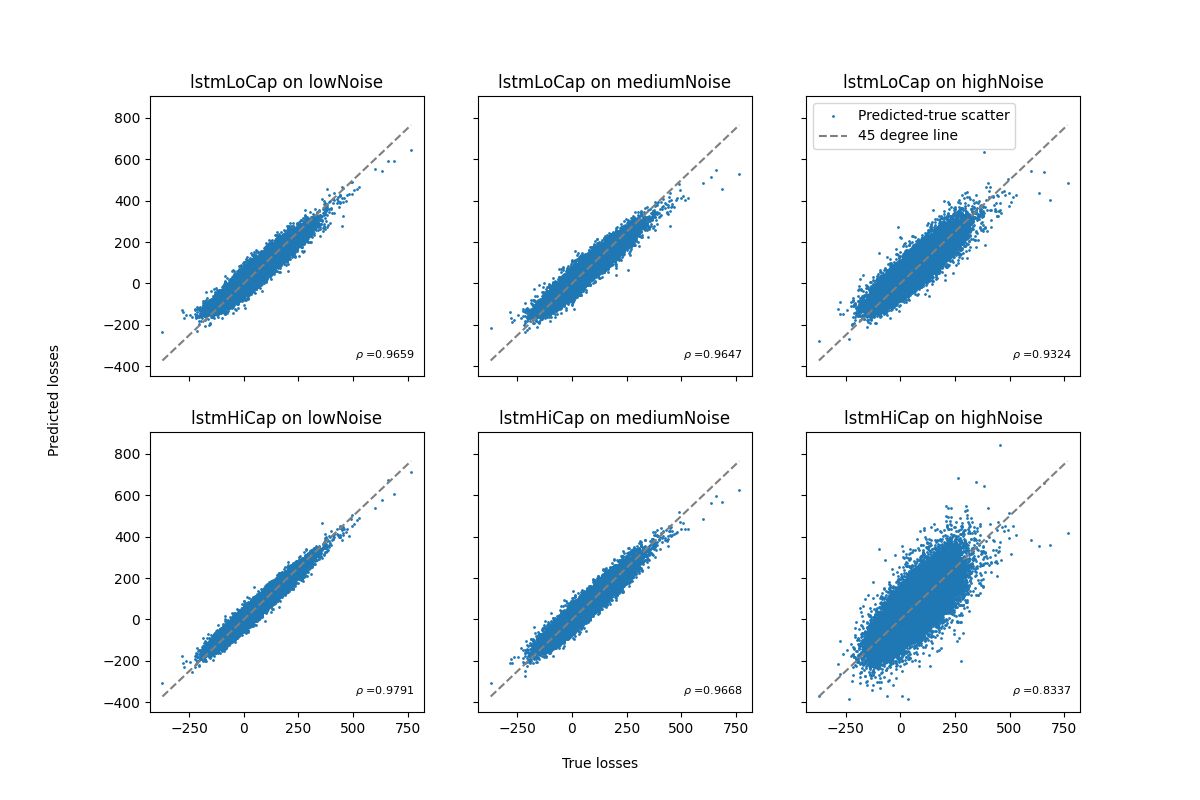
\includegraphics[width=\textwidth]{./project2/figures/qqPlots/lstmAll.png}
    \caption{QQ-plots between true losses (x-axis) and predicted losses (y-axis) for two LSTM metamodels.} 
    \label{fig2:QQ_All}
\end{figure}

In more details, the QQ-plots depicted in Figure~\ref{fig2:QQ_All} illustrates the fit of the two LSTM metamodels when different noise levels are present in the training labels.
They are arranged in a 2-by-3 grid, where the two rows correspond to the two LSTM metamodels with different model capacities, and the three columns correspond to the increasing noise levels.
The Pearson correlation coefficient between the true losses and the predicted losses is labeled in each subplot.
The sparsity of the plot increases as we move from left to right, indicating that the noise level in the training labels increases.
There are two key findings.
\begin{enumerate}
    \item   Compared to that of the regular LSTM, the metamodel predictions of high-capacity LSTM align more closely with the true losses when trained on the low-noise dataset.
    This is expected because the high-capacity LSTM has more trainable parameters and is able to learn more complex relationships better when the noise level is low.
    \item   When the noise level is medium or high, the high-capacity LSTM is more affected than the regular LSTM.
    This is because the high-capacity LSTM has more trainable parameters and is more prone to over-fitting to the noise in the training labels.
    In contrast, the regular LSTM is more robust to label noise.
\end{enumerate}

To further test the sensitivity of a LSTM metamodel and provide a more comprehensive picture of the noise tolerance of deep neural network models, we conduct a sensitivity analysis on the noise tolerance of the regular LSTM metamodel by varying the numbers of outer scenarios ($M$) and inner replications ($N$) used to generate the training data.
The number of outer scenarios corresponds to the number of data points in the training dataset, and the number of inner replications controls the noise level in the training labels.

\begin{table}[ht!]
    \small
    \centering
    \begin{tabular}{lccccc}
        \toprule
                            & $N=1$ & $N=10$  & $N=100$ & $N=\num{1000}$\\
        \midrule
        $M = 100$           & $1.139$ & $0.229$ & $0.167$ & $0.158$ \\
        $M = \num{1000}$     & $0.559$ & $0.173$ & $0.123$ & $0.127$ \\
        $M = \num{10000}$    & $0.283$ & $0.115$ & $0.099$ & $0.097$ \\
        $M = \num{100000}$   & $0.126$ & $0.068$ & $0.063$ & $0.063$ \\
        \bottomrule
    \end{tabular}
    \caption{MSE between regular LSTM predicted losses and true losses.}
    \label{tab2:lstm_sens}
\end{table}

\begin{table}[ht!]
    \small
    \centering
    \begin{tabular}{lccccc}
        \toprule
                          & $N=1$ & $N=10$  & $N=100$ & $N=\num{1000}$\\
        \midrule
        $M = 100$           & $0.764$ & $0.408$ & $0.131$ & $0.087$ \\
        $M = \num{1000}$     & $0.878$ & $0.367$ & $0.156$ & $0.087$ \\
        $M = \num{10000}$    & $0.351$ & $0.147$ & $0.064$ & $0.063$ \\
        $M = \num{100000}$   & $0.149$ & $0.065$ & $0.060$ & $0.038$ \\
        \bottomrule
    \end{tabular}
    \caption{MSE between high-capacity LSTM predicted losses and true losses.}
    \label{tab2:hicaplstm_sens}
\end{table}


Table~\ref{tab2:lstm_sens} and~\ref{tab2:hicaplstm_sens} show the average squared errors between the LSTM predictions and the true losses for increasing $M$ and $N$.
The last rows of Table~\ref{tab2:lstm_sens} and Table~\ref{tab2:hicaplstm_sens} show the performance of the regular and high capacity LSTM metamodels trained with $M=\num{100000}$ training labels with different noise levels.
We observe that an increasing $N$ reduces the MSE, but the reduction is not significant for a regular LSTM when $N$ is larger than $10$.
For the high-capacity LSTM, the MSE is significantly reduced when $N$ is increased from $1$ to $100$, but the reduction is not significant when $N$ is increased from $100$ to $\num{1000}$.
Another way to interpret the results in Table~\ref{tab2:lstm_sens} is to compare the MSEs for the same budget of $\Gamma = M \times N$. 
Entries on the same diagonal represents the same simulation budget.
For most budgets, the MSEs are also the lowest when $N = 10$.
The results in Table~\ref{tab2:lstm_sens} suggest that the performance of the LSTM metamodel is more sensitive to the number of outer scenarios than the number of inner replications.
Treating the neural network as an advanced regression metamodel, we find this pheonomenon to be consistent with the results in~\cite{broadie2015risk}, where the authors show that the performance of a regression-based nested simulation procedure is more affected by the number of outer scenarios.
The last row in Table~\ref{tab2:lstm_sens} and ~\ref{tab2:hicaplstm_sens} show that the high-capacity LSTM metamodel is relatively insensitive to the number of inner replications.
To make the most efficient use of a fixed simulation budget, the number of inner replication should be set constant around $N=10$ while increasing the number of outer scenarios to the maximum.

To further investigate the LSTM metamodels' sensitivity to data quantity and quality ($M$ and $N$, respectively), we report the Spearman rank correlation coefficients Table~\ref{tab2:lstm_corr}, which measure the ability to rank the scenarios by their true losses.
It is an appropriate measure of the metamodel's performance in the two-stage procedure, where the metamodel is used to identify the predicted tail scenario set, on which extensive simulations are run in stage 2 to estimate the $95\%$-CVaR.
The Pearson correlation coefficients are also included in the parentheses to illustrate the linear correlation between the predicted losses and the true losses.
They measure the metamodel's overall prediction accuracy.
The p-values of all quantities are less than $10^{-5}$, indicating that the correlations are statistically significant.


\begin{table}[ht!]
    \small
    \centering
    \begin{tabular}{lccccc}
        \toprule
                          & $N=1$        & $N=10$        & $N=100$       & $N=\num{1000}$ \\
        \midrule
        $M = 100$         & 0.638 (0.881) & 0.875 (0.915) & 0.896 (0.903) & 0.937 (0.941) \\
        $M = \num{1000}$   & 0.722 (0.768) & 0.899 (0.908) & 0.886 (0.891) & 0.922 (0.927) \\
        $M = \num{10000}$  & 0.845 (0.630) & 0.937 (0.900) & 0.908 (0.905) & 0.947 (0.948) \\
        $M = \num{100000}$ & 0.935 (0.640) & 0.963 (0.909) & 0.927 (0.922) & 0.965 (0.966) \\
        \bottomrule
    \end{tabular}
    \caption{Spearman (and Pearson) correlation coefficients between high-capacity LSTM predicted losses and true losses.}
    \label{tab2:lstm_corr}
\end{table}

Consistent with the results in Table~\ref{tab2:lstm_sens}, the Spearman correlation of the LSTM metamodel predictions with the true losses is insensitive to the number of inner replications, especially when $M$ is large.
The Pearson correlation coefficients are significantly lower for $N=1$ than the other $N$ values.

\begin{figure}
    \centering
    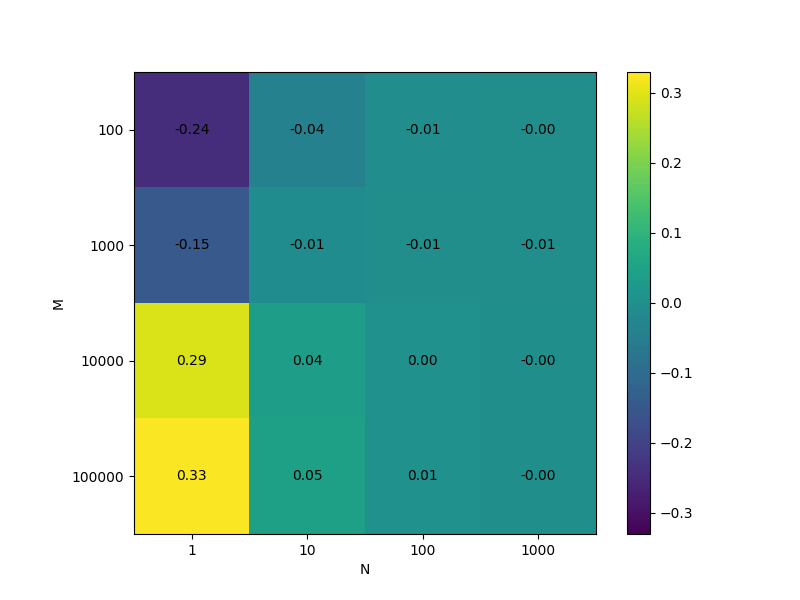
\includegraphics[width=0.6\textwidth]{./project2/figures/cor_heatmap.png}
    \caption{Difference between Spearman and Pearson correlation coefficients for high-capacity LSTM metamodel.}
    \label{fig2:cor-heatmap}
\end{figure}

Figure~\ref{fig2:cor-heatmap} shows the difference between the Spearman and Pearson correlation coefficients for the high-capacity LSTM metamodel.
The heatmap is generated by subtracting the Pearson correlation coefficients from the Spearman correlation.
We observe that Spearman correlation coefficients are not significantly different from the Pearson correlation coefficients for any $N$ larger than $10$. 
This is a strong evidence that the LSTM metamodel is not only able to effectively rank the scenarios by their true losses, but also able to make accurate loss predictions.
Instead of using the LSTM metamodel only for ranking in a two-stage procedure, LSTM's ability to cut through a moderate level of noise in training labels encourages us to use its predictions to estimate the CVaR directly. 

\subsection{Single-Stage Procedure}

The accuracy and robustness of the LSTM metamodels motivate us to propose a single-stage procedure that uses the metamodel predictions to estimate the CVaR directly. 
Instead of relying on the standard nested simulation procedure in Stage 2, the single-stage procedure is more efficient and extends to estimating other risk measures that require knowledge of the entire loss distribution.
In this section, we compare the single-stage procedure to the two-stage procedure and the standard procedure in estimating the $95\%$-CVaR of the hedging losses for GMWB.
% , and we also examine the single-stage procedure's performance in estimating the standard deviation of the hedging losses. 
In our numerical experiments, the results for the single-stage procedure is obtained with the same metamodels as in the two-stage procedure.
The only difference from Section~\ref{subsec:twoStageProcedure} is that the metamodel predictions are used to estimate the risk measures directly.

\begin{figure}[ht!]
    \centering
    \begin{subfigure}{0.48\textwidth}
        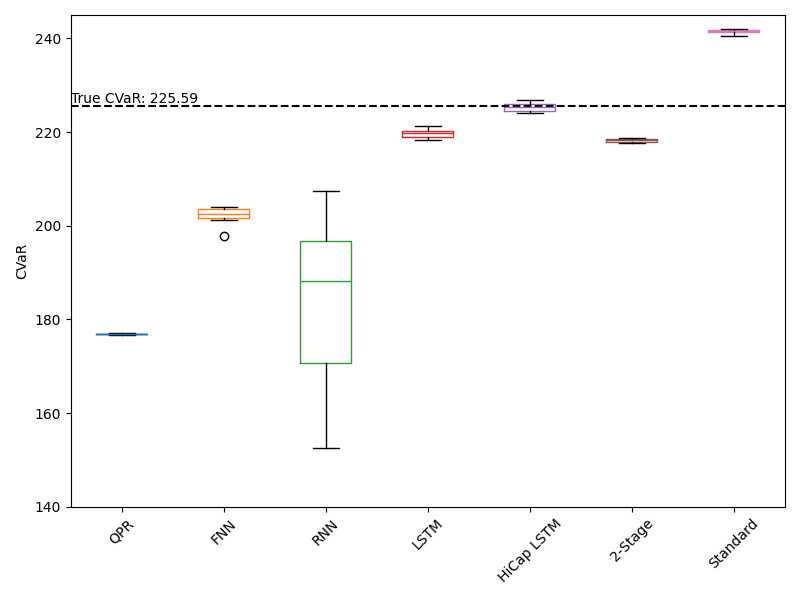
\includegraphics[width=\textwidth]{./project2/figures/singleStage/CVaRmediumNoise.png}
        \caption{Medium noise training labels ($N=10$)}
    \end{subfigure}
    \begin{subfigure}{0.48\textwidth}
        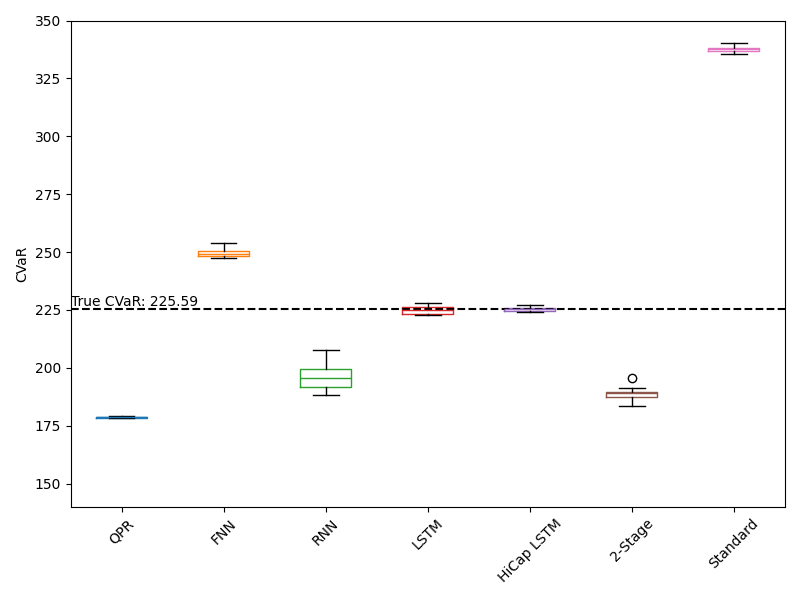
\includegraphics[width=\textwidth]{./project2/figures/singleStage/CVaRhighNoise.png}
        \caption{High noise training labels ($N=1$)}
    \end{subfigure}
    \caption{CVaR estimates of the single-stage procedure with metamodels.}
    \label{fig2:CVaRsingleStage}
\end{figure}

Figure~\ref{fig2:CVaRsingleStage} shows the boxplots of the 95\%-CVaR estimates of the single-stage procedure with different metamodels and compares them to the two-stage procedure and the standard procedure.
The two-stage procedure uses the same simulation budget as the single-stage procedure in Stage 1 with extra budget for extensive inner simulation on the predicted tail scenarios in Stage 2.
The metamodel with the best performance in the two-stage procedure is chosen, and the safety margin is set to 0\%.
The standard procedure shown in Figure~\ref{fig2:CVaRsingleStage} uses the noisy loss labels in the training dataset to estimate the CVaR directly, which uses the same simulation budget as the single-stage procedure.
We observe that the single-stage procedures with the LSTM metamodels consistently produce CVaR estimates that are closer to the true value than the standard procedure's estimate, especially when the noise level is high in the training labels.
It is another strong evidence that the LSTM metamodel is able to cut through the noise in the noisy training labels and make accurate loss predictions that lead to accurate CVaR estimates.
The difference in performance among the metamodels is more pronounced in the single-stage procedure than in the two-stage procedure.
Trained using low noise and medium noise labels, high-capacity LSTM metamodel consistently produces CVaR estimates that are closer to the true value than the regular LSTM, while the other metamodels produce even worse estimates.
Since we are using the metamodel predictions to estimate the CVaR directly without any safety margin, the metamodel's overall prediction accuracy becomes more important.
In other words, the single-stage procedure is more sensitive to the metamodel's ability to make accurate loss predictions than the two-stage procedure.
Previously, a generic FNN metamodel performs well in the two-stage procedure. 
However, results in Figure~\ref{fig2:CVaRsingleStage} suggest that the FNN metamodel should not be used in the single-stage procedure.

A single-stage procedure with a high-capcity LSTM metamodel is particularly superior to the two-stage procedure, as it is able to achieve a similar accuracy as the standard procedure with a much smaller simulation budget.
Note that the single-stage procedure does not require a safety margin.
By avoiding the calibration of the safety margin, it is more straight-forward to implement and is more efficient than the two-stage procedure.
For a two-stage procedure with a 0\% safety margin, the extra computational cost is from the extensive inner simulation in Stage 2.
On 4 20-core Intel Xeon Gold 6230 processors, Stage 2 of the two-stage procedure takes 30 minutes to run with parallel processing, while the 95\% confidence interval of training time of the high-capacity LSTM metamodel is $(19.64 \pm 0.94)$ minutes on a Nvidia RTX 3060 Ti GPU.
While the accuracy of the two-stage procedure is highly dependent on the safety margin, increasing the safety margin introduces extra computational cost.
Therefore, while achieving a higher accuracy in estimating the CVaR, the single-stage procedure requires only $60\%$ computation time of the two-stage procedure.

\begin{figure}[ht!]
    \centering
    \begin{subfigure}{0.48\textwidth}
        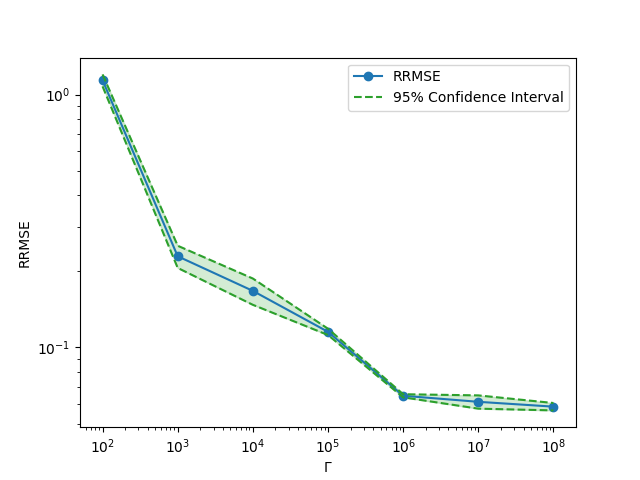
\includegraphics[width=\textwidth]{./project2/figures/singleStage/MSEConvergence_lstmLoCap.png}
        \caption{regular LSTM}
        \label{subfig2:convLoCap}
    \end{subfigure}
    \begin{subfigure}{0.48\textwidth}
        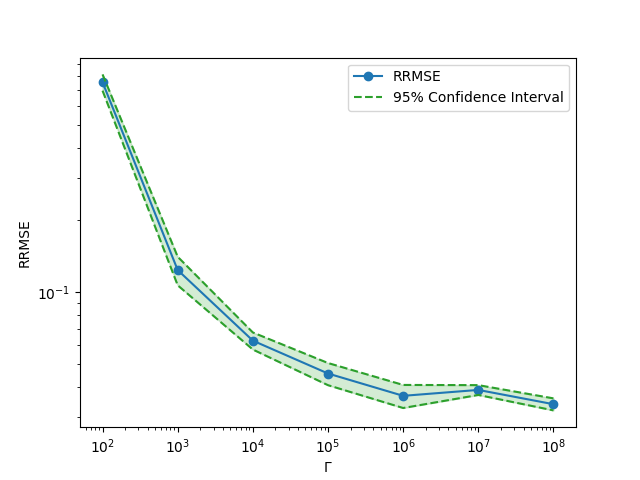
\includegraphics[width=\textwidth]{./project2/figures/singleStage/MSEConvergence_lstmHiCap.png}
        \caption{high-capacity LSTM}
        \label{subfig2:convHiCap}
    \end{subfigure}
    \caption{Empirical convergence of CVaR for the single-stage procedure with LSTM metamodels.} 
    \label{fig2:gammaConvergence}
\end{figure}


To further investigate the single-stage procedure's performance, we conduct a convergence analysis on the LSTM metamodels.
Figure~\ref{fig2:gammaConvergence} shows the log-log plots of the relative root mean square errors (RRMSE) between the LSTM metamodel CVaR predictions and the true CVaR against the total simulation budget $\Gamma$.
For each budget $\Gamma$, the metamodels are trained for different combinations of $M$ and $N$, and the metamodel with the best RRMSE is plotted.
While numerical results suggests that the CVaR estimator of the single-stage procedure with LSTM metamodels may have better accuracy than the two-stage procedure and the standard procedure when the number of outer scenarios is further increased, we found it difficult to compare their performance due to insufficient computational resources.
For $\Gamma \leq \num{100000}$, the number of outer scenarios is fixed at $M = \num{100000}$, and only the number of inner replications is varied.
Instead, we try to analyze the effect of the number of outer scenarios and the number of inner replications separately by fixing one and varying the other.

\begin{figure}[ht!]
    \centering
    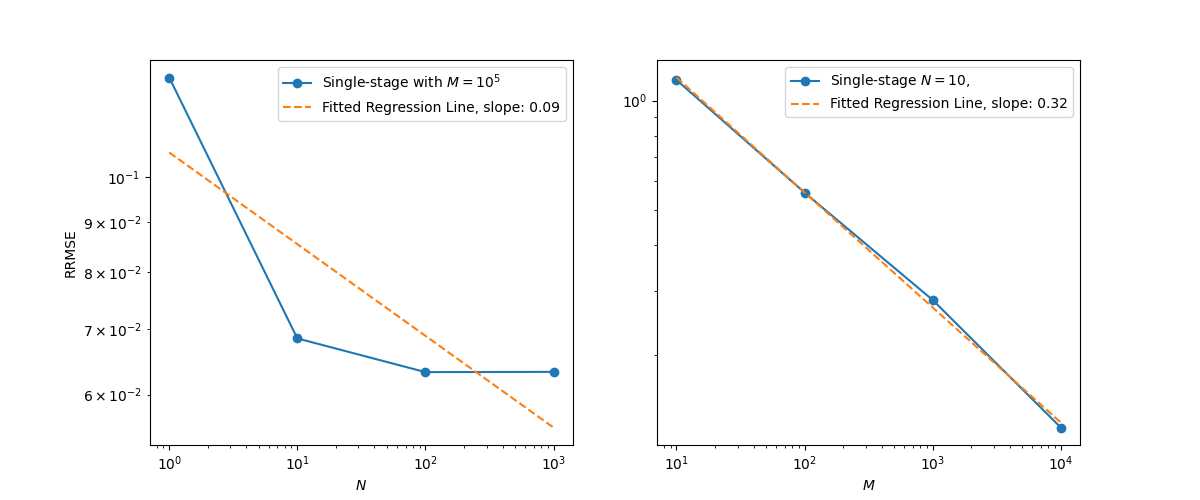
\includegraphics[width=\textwidth]{./project2/figures/singleStage/MSEConvergence_lstmLoCap_MN.png}
    \caption{Empirical convergence of the single-stage procedure with a LSTM metamodel.} 
    \label{fig2:mnConvergence}
\end{figure}

Figure~\ref{fig2:mnConvergence} shows the log-log plots of the RRMSE between the LSTM metamodel CVaR predictions and the true CVaR against the simulation budget.
The left figure shows the empirical convergence of the RRMSE for increasing inner replications with a fixed number of outer scenarios ($M=\num{100000}$), and the right figure shows the empirical convergence of the RRMSE for increasing outer scenarios with a fixed number of inner replications ($N=10$).
Due to computational constraints, we are not able to run the two-stage procedure and the standard procedure with more outer scenarios or more inner replications, therefore the comparison between the single-stage procedure is only available up to $M = \num{100000}$ and $N = \num{1000}$.
We observe that the RRMSE decreases as the simulation budget increases, and the rate of convergence is higher when the quantity of the data increases.
For an LSTM metamodel, increasing the data quality of the training labels has diminishing returns, which is consistent with the results in Figure~\ref{fig2:mnConvergence}.
For an increasing number of inner replications with fixed number of outer scenarios, the RRMSE cease to decrease after reaching $N = 100$. 
More specfically, when the quality of the training labels is fixed at $N = 10$, the CVaR estimator of single-stage procedure with a LSTM metamodel converge roughly in the order of $\mathcal{O}(M^{\frac{2}{3}})$.
This observation resonates with the convergence rate of a regression-based nested simulation procedure in~\cite{broadie2015risk}.
Hence, in practice, we suggest to run the single-stage procedure with a moderate number of inner replications and a large number of outer scenarios to achieve a high level of accuracy with a reasonable computational cost.

\section{Conclusion} \label{sec2:conclusion}
The proposed nested simulation procedures with deep neural network metamodels result in substantial computational savings in estimating CVaR of the hedging loss of a VA contract from accurately predicting the hedging losses and identifying the tail scenarios.
When new outer scenarios are generated, a trained LSTM metamodel can distinguish between tail and non-tail scenarios and make accurate predictions without the need to run new inner simulations.
Our novel experiment design allows us to examine the impact of label noise on deep neural network models.
We find that a deep neural network with a suitable architecture is able to cut through the noise in training labels and learn the true complex dynamic hedging model.
By showcasing the resilience of these models, our study aims to influence regulatory bodies towards recognizing the value and applicability of deep learning metamodels in financial risk management, and it provides informed suggestions and guidance for the incorporation and oversight of advanced deep learning metamodel in Monte Carlo Simulation in financial applications.
Our findings are particularly insightful in this context.
In our numerical experiments, a LSTM metamodel is resilient to a high level of noise in training labels and is able to make accurate predictions. 
This is a promising evidence that deep neural network metamodels can be used to improve the efficiency of Monte Carlo simulation for quantitative risk management tasks that require a computational-expensive simulation procedure.
We propose two nested simulation procedures that use deep neural network metamodels to estimate risk measures of the hedging loss of a VA contract.
For estimating tail risk measures, our two-stage procedure is designed to address regulatory concerns by avoiding the direct use of metamodel predictions but instead use them to identify the potential tail scenarios.
An extensive inner simulation is performed to achieve a high level of accuracy on the predicted tail scenarios.
However, the safety margin in the two-stage procedure is a user's choice and is not easy to determine before running extensive numerical experiments.

Our single-stage procedure uses the metamodel predictions to estimate the risk measure directly.
It is more efficient and can be extended to estimate risk measures that require knowledge of the entire loss distribution.
Our numerical experiments demonstrate that the proposed single-stage procedure with deep neural network metamodels result in further computational savings over our two-stage procedure. 
Furthermore, our numerical results provide evidences for adopting deep neural network metamodels in Monte Carlo simulation for risk management tasks.
Through our systematic study of the noise tolerance of deep neural network metamodels, we address regulatory concerns by showing that a LSTM metamodel is resilient to a high level of noise in training labels and is able to make accurate predictions.
A possible future research direction is to apply deep neural network metamodels in other financial risk management tasks that requires complex nested simulation with high-dimensional outer scenarios.
Another future research direction is to investigate the impact of label noise on other deep learning models, such as convolutional neural networks and transformer models, and to compare their performance with LSTM metamodels in nested simulation procedures. 
From a practical standpoint, the choice of a suitable deep neural network architecture is crucial for the success of a deep learning metamodel in nested simulation procedures.
We find that a LSTM metamodel is the most suitable for our dynamic hedging simulation model with time series features, but the optimal network architecture may vary for different simulation models.
Exploring deep neural network metamodels in other complex risk management tasks presents a promising avenue for research, especially as these tasks often involve complex, high-dimensional scenarios where traditional methods are insufficient. 
The versatility of neural networks could unlock new insights across a broad spectrum of financial and actuarial applications.

In this chapter, we have demonstrated the potential of deep neural network metamodels in nested simulation procedures for delta hedging of variable annuity contracts and have shown that they can be used to estimate risk measures with high accuracy and efficiency.
We have assumed a zero transaction cost model for our monthly rebalancing.
In practice, transaction costs can be significant and can affect the hedging strategy.
In the next chapter, we will extend our study to include transaction costs in the hedging strategy and investigate the impact of transaction costs on the hedging performance and the risk measures of the hedging error.
We will also explore the use of deep neural network models as reinforcement learning agents to optimize the hedging strategy by directly interacting with the financial market and maximize the hedging performance.